\chapter{Sulle Stelle di Neutroni}

Landau-Oppenheimer-Volkoff (LOV) ipotizzarono il concetto di una palla di neutroni: più pesanti degli elettroni, e quindi più lenti, avrebbero avuto una configurazione relativistica più compatta. 
Calcolarono che oggetti simili dovrebbero avere una massa limite di circa $5/6 M_{\odot}$, che considerando la GR è in realtà $M_{lim}^{GR}\simeq 3M_{\odot} $.
Furono inoltre in grado di prevedere che avrebbero dovuto emettere con spettro termico in banda X, a una temperatura di $T\sim10^7K$ (come al centro del sole, ma in superficie!!).

\section{Sullo spettro di emissione}
Per una stella di neutroni, la luminosità sarà data dalla \eqref{eq: luminosità di accrescimento NS} valutata per $R=R_{NS}$; se poi consideriamo il flusso di energia di un corpo nero, la luminosità ad esso corrispondente sarà:
\begin{equation}
    L=\sigma T^44\pi R^2,
\end{equation}
e le uniamo, si trova una temperatura pari a
\begin{equation}
    T=\left( \frac{GM\dot{M}}{4\pi R^3\sigma} \right)^{1/4}.
    \label{eq: Temperatura funzione di accrescimento}
\end{equation}
Nonostante la dipendenza sia piccola, servirebbe un valore tipico di $\dot{M}$ per trovare una stima di questa temperatura; ad esempio, possiamo usare il \textbf{limite di Eddington}.

\subsubsection{Limite di Eddington}
Sappiamo che, nell'atomo di H, i livelli energetici sono ben precisi: le frequenze sono esatte, ed è coinvolto l'intero atomo. 
Per ogni altra frequenza, l'atomo è trasparente.
Eddington notò che questo è vero finché non si considera l'interazione tra la radiazione e gli elettroni. 
In altre parole, non si può trascurare il fatto che, in una stella, gli elettroni degli atomi "parlano" con la radiazione.
Ricordiamo in questo senso che la sezione d'urto di Thomson per gli elettroni vale
\begin{equation}
    \sigma_{th,e} = \frac{8\pi}{3}\left(\frac{e^2}{m_ec^2}\right)^2=4\times10^{6}\sigma_{th,p}\hspace{1mm}.
    \label{eq: sezione d'urto Thomson}
\end{equation}
Per via del grande rapporto di massa con i protoni, la pressione di radiazione si esercita principalmente sugli elettroni.
Gli elettroni, quindi, parlano con la radiazione a \textit{tutte le frequenze}.
Inoltre, se anche l'atomo è ionizzato, spariranno tutte le righe di assorbimento ma non cambia assolutamente niente dal punto di vista della radiazione.
Tuttavia, nel momento in cui gli elettroni sono legati, nell'atomo di H, ai protoni, si comportano come delle particelle con \textbf{sezione d'urto} dettata dall'\textbf{elettrone}, e \textbf{massa} dettata dal \textbf{protone}.
Ricordando che il vettore di Poynting, il  cui modulo è il flusso della radiazione, è definito come $|\vec{S}|= \phi = \epsilon c $, dove $\epsilon$ è la densità di energia, vediamo che la pressione di radiazione esercitata sulla materia è data da
\begin{equation}
    P_{rad} = \frac{|\vec{S}|}{c}=\epsilon.
\end{equation}
Di conseguenza, su una superficie pari alla $\sigma_{th,e}$, la forza esercitata sarà:
\begin{equation}
    F=\frac{\phi}{c}\sigma_{th,e}=\frac{L}{4\pi r^2}\frac{\sigma_{th,e}}{c},
\end{equation}
considerando il flusso di una stella.
La materia di una stella, quindi, sarà contesa da una forza gravitazionale, e una forza della radiazione che spinge le particelle (da considerarsi di massa $m_p$), e al limite, queste due forze saranno uguali (oltre la stella si smembrerebbe a causa della pressione di radiazione troppo intensa):
\begin{equation}
    \frac{L}{4\pi r^2}\frac{\sigma_{th,e}}{c} = \frac{Gm_pM}{r^2},
\end{equation}
da cui, sostituendo la \eqref{eq: sezione d'urto Thomson}:
\begin{equation}
    L_{edd}=\frac{3}{2}\frac{Gm_pm_e^2c^5}{e^4}M_{\odot}\frac{M}{M_{\odot}}\simeq 1,3\times10^{38}\frac{M}{M_{\odot}}\hspace{1mm}erg\hspace{1mm}s^{-1}.
\end{equation}
%Ora, per collegare questa luminosità a una massa, ricordiamo che per stelle di sequenza principale vale la relazione
%\begin{equation}
%    \frac{L}{L_{\odot}}\sim\left(\frac{M}{M_{\odot}}\right)^4,
%\end{equation}
%da cui si ricava che 
Nell'accrescimento, la pressione di radiazione bloccherà la materia che accresce, causando dei ritmi on-off di materia che cade e viene bloccata:
la materia piove come a "blob", e la radiazione ci passa attorno rallentandola, raggiungendo così un equilibrio.
Al limite, avremo infine
\begin{equation}
    \frac{GM}{R}\dot{M}=\frac{M}{M_{\odot}}\frac{GM_{\odot}}{R}\dot{M}=1,3\times10^{38}\frac{M}{M_{\odot}},
\end{equation}
da cui infine:
\begin{equation}
    \dot{M}_{edd} = \frac{1,3\times10^{38}}{GM_{\odot}}R \propto R\hspace{1mm}.
\end{equation}
In unità di masse solari l'anno, e con $R$ espresso in unità di $10^6cm$, raggio tipico delle NS, si trova quindi:
\begin{equation}
    \dot{M}_{edd}=1,5\times10^{-8}\frac{M_{\odot}}{yr}R_6\hspace{1mm}.
\end{equation}
Quanto detto finora vale anche per BH, per i quali si trovano luminosità di Eddington estreme dell'ordine di $\sim10^{48}erg/s $!!
Con i risultati ottenuti, possiamo infine confrontare la luminosità di corpo nero con la luminosità di accrescimento di un oggetto al limite di Eddington, trovando
\begin{equation}
    T=\frac{GM\dot{M}_{edd}}{4\pi R^3\sigma}\sim 1,5\times 10^{7}K\simeq 1KeV,
\end{equation}
usando la relazione $E=kT$, cioè che l'emissione dovrebbe ricadere nella \textbf{banda X}!.

\subsubsection{Caso dei buchi neri super-massicci (SMBH)}
Nel caso di oggetti estremamente massicci, come i SMBH, che arrivano a $10^6-10^8 M_{\odot}$, si trovano $\dot{M}_{edd,SMBH}=0,5\frac{M_{\odot}}{yr}$!!
Nel loro caso, inserendo nella \eqref{eq: Temperatura funzione di accrescimento} questo valore, e sostituendo $R\longleftrightarrow R_{sch}$, si trovano temperature molto più basse:
\begin{equation}
    T_{BH}\simeq 10^3K,
\end{equation}
per cui potremmo aspettarci emissione \textbf{in ottico}, esattamente come accade per le normali stelle, ma con luminosità assurde per oggetti a distanze enormemente grandi (note dallo shift delle righe di assorbimento): da questo, il nome "quasi-star", o QUASAR.


\subsection{Pulsar}
Nel '67 Jocelyn Bell osservò una strana regolarità nel segnale radio, che inizialmente interpretò come LGM (little green man, alieni).
Sfortunatamente, o fortunatamente, si trattava di tutt'altro.
Iniziarono a nascere dei modelli, per interpretare questo segnale con un periodo di $\sim1s$.

\subsubsection{Cosa poteva causare questa periodicità?}
Doveva essere un oggetto rigido, con periodo T, di piccola dimensione e grande densità.
Poteva essere descritto come un pendolo?
In quel caso il periodo sarebbe $T=\sqrt{\frac{R}{g}} = \sqrt{\frac{R^2}{GM}} $: la massa dovrebbe essere enorme, ed il raggio molto piccolo, per un periodo così breve.
Questo portò a rifarsi alle già ipotizzate NS, che avevano le carte in regola per essere buone candidate: grande densità e piccolo raggio.
Un aspetto del pendolo, e dell'oscillazione come fenomeno periodico, è che perdendo energia l'oscillazione diminuisce di ampiezza, ma il periodo rimane costante.
Tuttavia, con la tecnica dell'\textit{epoch folding}, si scoprì l'incredibile stabilità del segnale su breve scala, ma anche che su tempi lunghi il periodo si allungava leggermente! 
Le oscillazioni o vibrazioni erano da escludere.
Nacque così l'ipotesi di una sfera con un punto luminoso, che ruota su se stessa\footnote{Si vedano \cite{Pacini}, \cite{Gold}, \cite{Ostriker_Gunn} e \cite{Goldreich_Julian}.}.

\subsubsection{Emissione nel radio}
Come detto, l'emissione scoperta da Jocelyn Bell era nello spettro radio. 
Si ricordi che, nella radiazione di corpo nero corrispondente a una temperatura T,
\begin{equation}
    B_{\nu} = \frac{8\pi h}{c^3}\frac{\nu^3}{e^{-\frac{h\nu}{kT}} - 1},
\end{equation}
la frequenza corrispondente al picco è data da
\begin{equation}
    \nu_{max}= \frac{c}{\lambda_{max}}=\frac{3kT}{h}.
    \label{eq: picco Black Body}
\end{equation}
Ora, se all'emissione in X corrisponde $1KeV$, cioè circa $10^6K$, considerando che $\nu_X\sim 3\times10^9\nu_{radio} $ si avrà che a un'emissione termica in radio corrisponde una \textit{temperatura di brillanza}\footnote{La temperatura di brillanza è la temperatura che dovrebbe avere un oggetto di cui osserviamo un emissione ad una data frequenza, se questo emettesse perfettamente come un corpo nero piccato a quella frequenza.} pari a $T_{radio}\sim3mK$, inferiore alla temperatura del fondo cosmico!
Ponendo che la frequenza che osserviamo (radio, $\sim GHz$) corrisponda al picco di un corpo nero, la temperatura che questo dovrebbe avere esce senza senso. 
Si potrebbe quindi ipotizzare che ciò che stiamo osservando sia una coda della curva di corpo nero, e quindi le possibilità sarebbero due:
\begin{itemize}
    \item stiamo osservando una frequenza \textit{oltre} il massimo, ma in questo caso sarebbe anche peggio. Infatti, se la frequenza del massimo fosse anche più piccola di quella osservata, la temperatura risulterebbe anche più piccola!
    \item stiamo osservando una frequenza prima del picco, ma in questo caso dovrei vedere molta più emissione a frequenze più elevate, in quanto l'intensità cresce come $\nu^2$ fino al raggiungimento del picco.
\end{itemize}
Detto questo, di pulsar termiche ne esistono, ma solamente negli X!
Questa considerazione consentì di escludere l'accrescimento, e di ipotizzare uno spettro non termico.
PARTE DA INTEGRARE, SU COME CAPIRONO CHE SI TRATTAVA DI SINCROTRONE, E FA RICHIAMO DI COSA SIA SINCROTRONE.

\subsection{Sui campi magnetici}
Conseguenza: i campi magnetici dovevano essere enormi!
Tuttavia, sappiamo che $div\vec{B}=0$, e che i campi magnetici possono essere generati solo da cariche in movimento: 
le NS non possono essere solo neutroni, servono cariche.
Deve esistere una popolazione di protoni ed elettroni che si formano e distruggono statisticamente, attratti da una gravità così forte che estrarli dev'essere molto difficile.
Se però la NS, con il suo campo magnetico, ruota sufficientemente veloce, si genererà un campo elettrico sufficientemente forte da strappare gli elettroni (i protoni, $2000$ volte più pesanti, restano incollati dalla gravità).
\subsubsection{Dipolo magnetico e "Larmor" magnetico}
Immaginiamo di poter descrivere il campo magnetico di una pulsar come un dipolo magnetico perfetto: la rappresentazione più corretta sarebbe quindi un solenoide attraversato da corrente.
Fregandocene di cosa ci sia dentro a generarlo, per ora ci interessa capire cosa succeda al campo in sé concettualmente.
Sappiamo che una carica elettrica accelerata emette radiazione, secondo la formula di emissione di Larmor:
\begin{equation}
    L=\frac{2}{3c^3}q^2a^2=\frac{2}{3c^3}q^2|\ddot{x}|^2=\frac{2}{3c^3}|\ddot{d}|^2,    
\end{equation}
dove $d=qx$ è il momento di dipolo elettrico.
Per una analogia brutale, la cui giustificazione matematica non ci interessa in questo momento, si può scrivere una formula che funzioni allo stesso modo, ma con il momento di dipolo magnetico:
\begin{equation}
    L=\frac{2}{3c^3}\ddot{\mu}^2,
\end{equation}
dove $\mu = B_{eq}R^3$.\footnote{Si ricordi che il campo di dipolo è definito come
\begin{equation}
    B(r)=-\nabla\Psi=\frac{1}{4\pi}\left( \frac{3\vec{r}(\vec{\mu}\cdot\vec{r})}{r^5} - \frac{\vec{\mu}}{r^3}\right),
\end{equation}
dove $\Psi=\frac{\vec{\mu}\cdot\vec{r}}{4\pi r^3} $ è il potenziale magnetico scalare. 
Quindi si hanno i seguenti casi:
\begin{itemize}
    \item se $\mu\parallel r\xrightarrow{}B(r)=\frac{1}{4\pi}\frac{2\mu}{r^3}$,
    \item se $\mu\perp r\xrightarrow{}B(r)=-\frac{1}{4\pi}\frac{\mu}{r^3}$.
\end{itemize}
Si noti che, in c.g.s., il fattore $\frac{1}{4\pi}$ sparisce.
}
In effetti, immaginando di tagliare il campo di un dipolo con una sfera di raggio pari al raggio del solenoide che genera il campo, troveremmo che le linee di questo saranno perpendicolari al piano equatoriale della sfera, come si vede in \textbf{Figura \ref{fig:momento di dipolo ns}}.
\begin{figure}[h!]
    \centering
    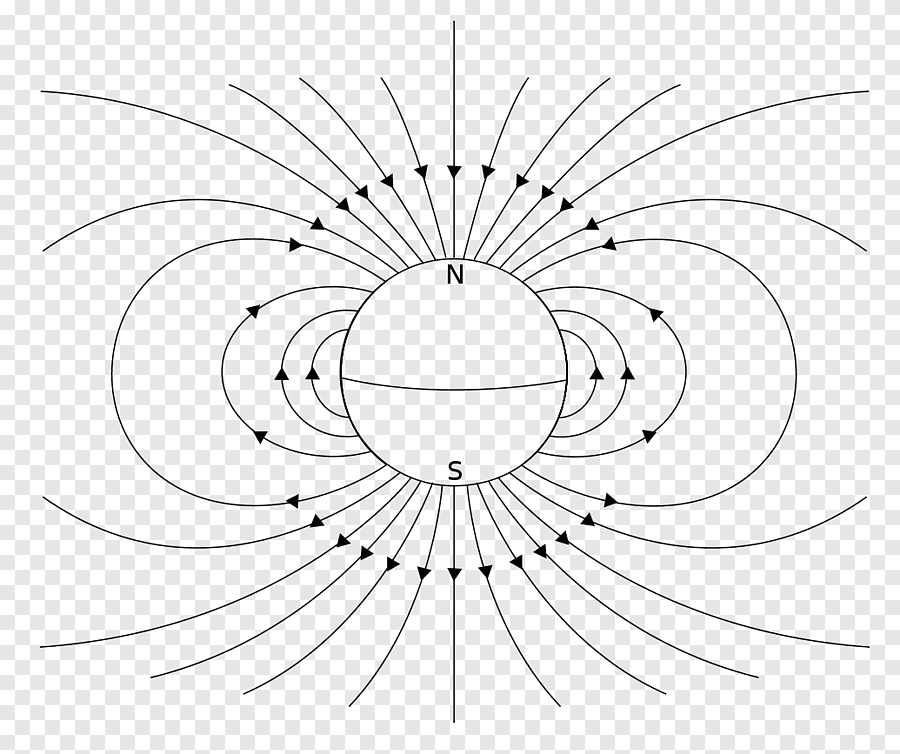
\includegraphics[width=0.4\linewidth]{Immagini/dipole_moment.png}
    \caption{Campo magnetico di un dipolo per una stella di neutroni.}
    \label{fig:momento di dipolo ns}
\end{figure}
Dalla definizione di dipolo magnetico, troviamo che il campo equatoriale alla superficie della NS sarà
\begin{equation}
    B_{eq,S_{NS}} = \frac{\mu}{R_{NS}^3},
\end{equation}
mentre al polo il campo sarà
\begin{equation}
    B_{pol,S_{NS}}=\frac{2\mu}{R_{NS}^3}.
\end{equation}
Inoltre, poiché il campo al polo ha verso opposto al campo equatoriale, come si vede in \textbf{Figura \ref{fig:momento di dipolo ns}}, uno sarà concorde e l'altro discorde con $\mu$.
\subsubsection{Facciamo ruotare il sistema}
A questo punto, se la stella di neutroni sta ruotando attorno a una direzione che forma un angolo $i$ con la direzione del dipolo, possiamo scomporre nelle direzioni ortogonale e parallela il momento, come $\vec{\mu}=\vec{\mu}_{\perp}+\vec{\mu}_\parallel $, dove
\begin{align}
   \mu_{\perp} & =  \mu \sin{i}\\
   \mu_\parallel & =  \mu \cos{i}\hspace{1mm}.
\end{align}
Durante la rotazione, la componente perpendicolare varierà direzione nel piano equatoriale $[x,y]$ continuamente, mentre la componente parallela resterà invariata: $\ddot{\mu_\parallel}=0$, e quindi
\begin{align}
    \ddot{\mu}^2_{\perp}&=\ddot{\mu}_{\perp,x}^2+\ddot{\mu}_{\perp,y}^2\notag\\
    &= \mu^2\Omega^4\sin^2{i}\cos^2{\Omega t}+\mu^2\Omega^4\sin^2{i}\sin^2{\Omega t}\notag\\
    &= \mu^2\Omega^4\sin^2{i},
\end{align}
e quindi
\begin{equation}
    \boxed{L=\frac{2}{3c^3}\mu^2\Omega^4\sin^2{i}}.
    \label{eq: emissione dipolo magnetico rotante}
\end{equation}
Questa è quindi l'emissione da un dipolo magnetico rotante, ma ci si chiede ora: questa energia a scapito di chi è?

\subsubsection{Energia cinetica rotazionale}
Il sistema avrà una energia cinetica rotazionale $E_{rot}=\frac{1}{2}I\Omega^2 $, dove $I=\frac{2}{5}M_{NS}R_{NS}^2 $ è il momento di inerzia della stella di neutroni (considerata omogenea).
L'emissione come dipolo, quindi, causerà una variazione di questa energia, che si calcola come
\begin{equation}
    \dot{E}_{rot}=I\Omega\dot{\Omega}+\frac{1}{2}\Omega\dot{I}=I\Omega\dot{\Omega},
    \label{eq: variazione energia rotazionale}
\end{equation}
dove $\dot{I}=\frac{2}{5}M_{NS}R_{NS}\dot{R_{NS}}+\frac{2}{5}R_{NS}^2\dot{M}_{NS } = 0$, se si assume che, a ordine zero, il raggio della stella di neutroni sia $\sim cost.$, dipendendo solo da $M_{NS}$, e che questa in prima battuta non vari.
Ora, notiamo che la \eqref{eq: variazione energia rotazionale} deve essere esattamente l'opposto della \eqref{eq: emissione dipolo magnetico rotante}, e uguagliando il lato destro delle due si trova infine\footnote{Si noti che la $\Omega$ la si conosce dalla misura di $\nu$ deqli impulsi, mentre la $I$ la valuto con valori tipici di raggio e il valore di Chandrasekar per la massa, e risulta quindi un parametro sperimentale.}
\begin{equation}
    \dot{\Omega}=-\frac{2}{3c^3}\frac{\mu^2\sin^2{i}}{I}\Omega^3.
    \label{eq: variazione vel. ang. per emissione di dipolo rotante}
\end{equation}
Tramite la derivata logaritmica\footnote{Se ad esempio si vuole derivare l'espressione
\begin{equation}
    G=a^\alpha b^\beta c^\gamma \dots p^\pi \cdot k
\end{equation}
dove $k$ è una costante, si può semplificare il conto usando il logaritmo:
\begin{equation}
    \frac{d\ln{G}}{dt} = \frac{d\ln{(a^\alpha b^\beta c^\gamma \dots p^\pi \cdot k)}}{dt}=\frac{d(\alpha\ln{a} + \beta\ln{b + \dots + \pi\ln{p} + \ln{k}})}{dt},
\end{equation}
per cui, ricordando che $\frac{d\ln{x}}{dt}= \frac{\dot{x}}{x}$, si trova infine
\begin{equation}
    \frac{\dot{G}}{G} = \alpha\frac{\dot{a}}{a} + \beta\frac{\dot{b}}{b}+\dots+\pi\frac{\dot{p}}{p}.
\end{equation}
}
, è quindi possibile trovare la relazione corrispondente nel periodo:
\begin{equation}
   - \frac{\dot{\Omega}}{\Omega}=\frac{\dot{P}}{P}=\frac{2}{3c^3}\frac{\mu^2\sin^2{i}}{I}\left(\frac{2\pi}{P}\right)^2,
\end{equation}
da cui
\begin{equation}
    P\dot{P}=\frac{8\pi^2}{3c^3}\frac{\mu^2\sin^2{i}}{I}.
    \label{eq: PPdot}
\end{equation}
Per prima cosa, si noti che per come lo abbiamo ricavato, $\dot{P}>0$, e in effetti è proprio ciò che si osserva.
In secondo luogo, si noti che $P$ e $\dot{P}$ li posso misurare direttamente, $I$ lo posso stimare, e posso prendere $\sin{i}\sim1$ (si ricordi che stiamo assumendo che $M_{NS}, R_{NS}\sim cost. $).
Questo modello prevede che le NS con campo magnetico polare rallentino, e consente di ottenere una misura (a ordine di grandezza) del campo lungo l'asse.
Il momento di inerzia della NS è enorme, il che rende l'oggetto estremamente stabile (come si vede dalla \eqref{eq: PPdot}, più $I$ è grande più piccola è la derivata, e quindi più stabile è il periodo).

\subsubsection{Valutazione del campo magnetico}
Nell'articolo \cite{Bhattacharya} si trova, a partire dalla \eqref{eq: PPdot}, e ricordando che $\mu = R^2_{NS}B_{eq,NS} $, che i campi sono $B_{NS,eq}\sin{i}=3,2\times10^{19/20}\sqrt{P\dot{P}} \hspace{1mm}G$.
Se ci sono campi così forti, questo dovrebbe avere un qualche effetto sulla struttura della NS. 
Infatti, i campi magnetici possono esercitare una \textbf{pressione magnetica}:
\begin{equation}
    P_{mag}\sim\frac{B^2}{4\pi},
    \label{eq: pressione magnetica}
\end{equation}
delle stesse dimensioni di una densità di energia.
L'energia gravitazionale, di contro,  è come se esercitasse una pressione in direzione verso l'interno, e posso confrontarla con l'energia corrispondente alla densità in \eqref{eq: pressione magnetica}:
\begin{equation}
    \frac{GM}{R}\sim\frac{B^2_{NS}}{4\pi}\frac{4\pi}{3}R^3,
\end{equation}
da cui si può porre un limite concettuale, superato il quale la NS si smembrerebbe, come
\begin{equation}
    B_{NS}\leq\left( \frac{3GM}{R^4} \right)^{1/2} \sim 10^{17}G.  
\end{equation}
Di conseguenza, affinché campi teoricamente dell'ordine di $10^{19}/10^{20}G$ scendano al di sotto di questo limite, occorre che $\sqrt{\dot{P}}$ sia un valore molto piccolo.
Prendiamo, ad esempio, la Crab, per la quale si misura $B=10^{19}\sqrt{P\dot{P}} = 10^{12} $: in questo caso occorrerebbe che $P\dot{P} = 10^{-15} $. Considerando che $P_{crab} = 33\cdot10^{-3}s$, allora si deve avere $\dot{P}_{crab}\sim10^{-14} $: per variare di $1s$, impiega circa $10^7yr$!\footnote{
Come calcolo $\dot{P}$?
Osservo un impulso oggi e, con il periodo P, posso misurare il numero di cicli che lo separano da un impulso tra, ad esempio, un anno, assumendo che il periodo sia rimasto costante. 
Posso quindi vedere di quanto arrivo in \textit{anticipo}.
So poi che $\Delta\phi = \frac{1}{2}\dot{P}\left(\frac{t}{P}\right)^2 $, con $t/P$ il numero di cicli, è il ritardo di fase che accumulo nell'anno trascorso: essendo un valore piuttosto grande, riesco ad apprezzarlo.
}
\subsection{Che cosa emette di fatto?}
Abbiamo descritto il sistema come un dipolo rotante che emette, ma fisicamente che cosa sta emettendo veramente?
Con i campi stimati $\sim10^{12}G$, la luminosità calcolata con la \eqref{eq: emissione dipolo magnetico rotante} risulta $L\simeq 1,3\cdot10^{38}erg/s \sim 10^5L_{\odot} $!\footnote{Questo è un buon momento per far notare che questa informazione la si è ricavata partendo solamente dall'assunzione che si trattasse di un grosso oggetto che ruota e rallenta, un po' di Fisica II e alcuni accorgimenti.}
Tutta questa luminosità, in che cosa viene emessa? Onde elettromagnetiche sì, ma in che frequenza?
Nota la frequenza di rotazione della NS, le onde saranno emesse a questa frequenza:
\begin{equation}
    \lambda = \frac{c}{\nu}= cP = 3\cdot10^{9}cm \simeq 10^4km,
\end{equation}
che è un valore confrontabile con il raggio della terra!
Sotto il radio non c'è altro nello spettro, quindi di definisce comunque emissione radio (ultra-low).
Si pensi che la corrente di rete elettrica è a $50Hz$, e queste onde sono emesse a $\sim30Hz$, quindi si tratta circa dello stesso tipo di onda. 
Onde simili sono usate nei sottomarini perché non vengono assorbite dall'$H_2O$.
\subsubsection{Queste onde come vengono generate?}
Le linee del campo magnetico della NS ruotano, solidali, con essa.
Questo significa che una linea di campo a una certa distanza $r$ dalla stella, ruoterà con una velocità pari a $v_t=\Omega r$.
Si può intuire che, con $\Omega$ così grandi, la velocità tangenziale cresce, all'aumentare del raggio, fino a valori enormi, e farà presto a raggiungere un limite invalicabile: la velocità della luce.
Si definisce quindi il raggio limite di un cilindro, oltre il quale le linee di campo risulterebbero avere una velocità tangenziale superluminale, che prende il nome di \textbf{light cilinder}:
\begin{equation}
    r_{lc}=\frac{c}{\Omega}=\frac{cP}{2\pi}.
    \label{eq: raggio light cilinder}
\end{equation}
In effetti è come se si formasse un cilindro limite oltre cui le linee non possono più essere considerate solidali\footnote{Si noti che per la Crab, ad esempio, il light cilinder risulta di $\sim 10^8/10^9 cm$, laddove la NS ha raggio di $\sim10^6cm$}.
Ora, le linee variano nel tempo così tanto da generare $rotE = -\frac{1}{c}\frac{\partial B}{\partial t} $ e $rotB = \frac{1}{c}\frac{\partial E}{\partial t} $; al $r_{lc}$ variano talmente tanto che si genera un $\vec{E}$ indotto così intenso da uguagliare il $\vec{B}$ che lo ha generato:
da quel raggio in poi, ci sono due campi, uno elettrico e uno magnetico, che oscillano con eguale intensità, cioè onde elettromagnetiche!\footnote{\cite{Harding2022}}

\subsubsection{Radiazione di curvatura}
In un dipolo non rotante, le curve del campo magnetico si chiudono tutte, a raggi diversi, fatta eccezione per la linea verticale.
Le linee che arrivano al light cilinder di un dipolo rotante, invece, non potendolo superare non possono chiudersi, e restano dunque aperte.
A questo punto, se degli $e^-$ vengono strappati dalla superficie dalle enormi differenze di potenziale che si generano o se, a causa delle enormi energie (fotoni dell'ordine del $MeV$), si formano proprio delle coppie $e^+e^-$, le cariche negative vengono trasportate dalle linee di campo in una direzione, mentre le cariche positive nella direzione opposta, e vengono accelerate dalle linee di campo curve, emettendo quindi \textbf{radiazione di curvatura} fino a raggiungere emissioni dell'ordine dei $MeV$: a catena, questo genererà altre coppie di cariche che verranno accelerate nuovamente ed emetteranno nuovamente per curvatura, e così via.
Da una singola carica, a valanga derivano generazioni successive di cariche che emettono per curvatura.
\begin{figure}[h!]
    \centering
    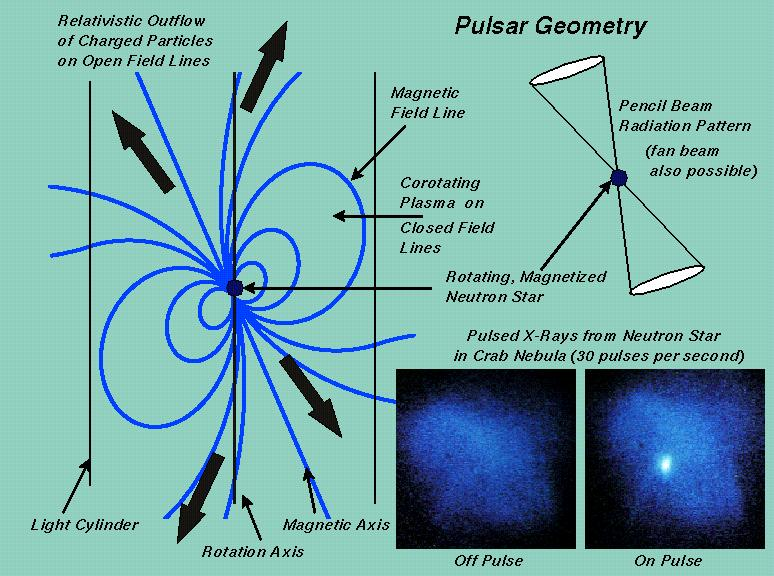
\includegraphics[width=0.5\linewidth]{Immagini/light cilinder.jpg}
    \label{fig: pulsar con light cilinder}
\end{figure}
Gli elettroni che vengono strappati dalla superficie, inoltre, formano delle nuvole di cariche che si spostano, come accade agli elettroni in un conduttore in campo elettrico esterno, e che generano a loro volta un nuovo campo elettrico che si oppone a quello indotto dalla rotazione.  
Quello che avviene in un conduttore è che, dopo un po' di tempo, la densità di corrente diventa complicatissima, ma fondamentalmente diventa tale da \textit{annullare} ogni componente del campo elettrico \textit{parallela} alla superficie. In questo caso avviene una cosa del tutto analoga, ma nel volume.\footnote{ \cite{Goldreich_Julian}}.
Le nuvole di cariche così formate ruotano solidali con la pulsar, e all'interno di questa densità di carica complicata si aprono dei \textbf{gap}, spazi vuoti che si comportano come delle specie di \textit{condensatori}.
All'interno delle zone cariche, il campo indotto rende il campo elettrico complessivo pari a $0$, mentre nelle gap, vuote, il campo elettrico non viene annullato!
In particolare, si può distinguere fra \textbf{inner gaps} e \textbf{outer gaps}, in base alla loro vicinanza dalla superficie della NS piuttosto che dalla loro distanza dal light cilinder.


\subsubsection{Emissione complessiva}
In \cite{Goldreich_Julian} è dimostrato che l'energia per unità di tempo persa dall'emissione dovuta alle cariche accelerate dalle linee di campo è $\propto \cos^2i$, e che è massima per un rotatore \textit{allineato}, e minima per un rotatore ortogonale
\begin{align}
    &L_{current}=\cos^2i\left( \frac{2}{3c^3}\mu^2\Omega^4 \right)\\
    &L_{wave}=\sin^2i\left( \frac{2}{3c^3}\mu^2\Omega^4 \right),
\end{align}
per cui
\begin{equation}
    L_{tot}=L_{wave}+L_{current}= \frac{2}{3c^3}\mu^2\Omega^4=I\Omega\dot{\Omega}.
\end{equation}
Ora, ricordando la \eqref{eq: PPdot}, e che $\mu = BR^3$, si può ottenere che 
\begin{equation}
    B=\sqrt{\frac{3c^3I}{8\pi^2R^6}P\dot{P}},
    \label{eq: B in funzione di PPdot}
\end{equation}
dove come si vede la dipendenza da $i$ se ne va:
l'oscillatore allineato emette tutta la potenza in correnti di cariche, e niente potenza in onde EM a bassa frequenza; il rotatore ortogonale viceversa emetterà solo onde EM a bassa frequenza, e niente in correnti; il rotatore generico, emetterà un po' in un modo e un po' nell'altro: una frazione $\propto\cos^2 {i} $, l'altra $\propto\sin^2 {i} $.
Se prima potevo stimare $B\sin{i}$, ora sono sicuro che, misurando $P$ e $\dot{P}$, posso stimare il campo esatto, che non dipende dall'inclinazione.

\subsection{Sulla Crab}
\subsubsection{Assorbimento del plerione}
Attorno alla Crab si trova il \textbf{plerione}, un tipo di nebulosa che si trova all'interno dell'involucro dei resti di supernova (SNR), alimentato dai venti generati dalla sua pulsar centrale. 
Questa nube ha una frequenza di plasma superiore ai $30Hz$, per cui mi aspetto che la radiazione elettromagnetica della pulsar all'interno non possa arrivare, venendo assorbita dalla nube.
La potenza dovuta agli elettroni relativistici penetra un po', ma quando poi incontra la Crab Nebula viene dissipata in essa, scaldandola.
La Crab scaldata, quindi, emette in ottico.
Pacini descrisse la nebula come un \textit{bolometro}, che raccoglie energia della NS e la riemette in altro modo. 
Dedusse che si può calcolare se, effettivamente, la Crab riemette un'energia davvero pari a $\sim10^{38}erg/s$.
Questa previsione può essere misurata direttamente!\footnote{Da $P\dot{P}$ si può dedurre il campo magnetico, ma non posso confrontare questa previsione con dei dati sperimentali: non posso misurarlo direttamente perché è un parametro interno della teoria.
Invece, infilando quello stesso campo in questa formula trovo una potenza che è svincolata da questa teoria, non ne è parametro.
Se la misuro e trovo lo stesso valore, la previsione della teoria è corretta, e sì che posso dire qualcosa!
In effetti, se dopo quasi 1000 anni emette ancora così tanto, qualcosa dentro ci dev'essere ad alimentarla.}\\
In effetti, le osservazioni confermano la previsione.
La coincidenza fra previsione e misure rende la teoria "giusta" e il parametro interno $B$ \textit{probabilmente} giusto.

\subsubsection{Ma allora che cosa si osserva?}
Se in teoria abbiamo capito il bilancio energetico dell'UV, ci si chiede allora dove nasca il \textit{radio}, e la risposta risiede nei gap:
come abbiamo accennato, nei gap non ci sono cariche, e se un gap è situato fra due regioni di cariche opposte, al suo interno il campo elettrico totale sarà $\not=0$. 
Si sviluppa quindi un processo a valanga di produzione di coppie che emettono fotoni a energie inizialmente elevate (che causano la valanga) ma che diventano successivamente sempre più basse, in quanto coppie generate all'inizio avranno più spazio per accelerare nella gap rispetto a coppie generate più avanti!
Ad ogni modo, si creano dei pacchetti lunghi anche centimetri\footnote{Si ricorda infatti, che l'emissione di un singolo elettrone accelerato è ridicolmente piccola, ma l'emissione di un pacchetto di $\sim10^{20}$ elettroni coerenti è estremamente amplificata (vedi \cite{Bradt}, ch. 8).} di cariche positive e negative che muovono in direzioni opposte.
Se la gap è \textit{esterna} questo funziona bene, perché la curvatura è ampia, mentre se è \textit{interna}, produrrà meno a causa della curvatura minore.
Tuttavia, se lungo una linea retta la carica ha una velocità leggermente inclinata (angolo di \textbf{pitch}) rispetto alle linee di campo, spiraleggierà, con una velocità angolare di \textbf{ciclotrone} pari a
\begin{equation}
    \Omega_{ciclo} = \frac{eB}{cm_e},
    \label{eq: ciclotrone}
\end{equation}
o, nel caso relativistico, in cui prende il nome di \textbf{sincrotrone}, pari a 
\begin{equation}
    \Omega_{sinc}=\frac{eB}{\gamma cm_e}.
    \label{eq: sincrotrone}
\end{equation}
Dalle gap interne, dunque, ci aspetteremmo un'emissione a questa frequenza, ma a velocità elevate un nuovo effetto prende piede: il \textbf{beaming}, fenomeno legato all'aberrazione relativistica, che concentra l'emissione di una sorgente, ad esempio isotropa se a riposo, in un cono molto stretto lungo la direzione del moto
\begin{figure}[h!]
    \centering
    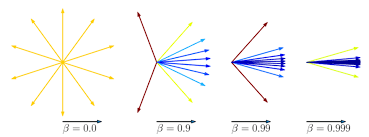
\includegraphics[width=0.5\linewidth]{Immagini/beaming iso source.png}
    \label{fig: beaming sorgente isotropa}
\end{figure}.\\
Questo fenomeno fa emergere un ulteriore fattore $\gamma$, e si manifesta come una serie di flash di durata $\propto 1/\gamma$, distanziati di un periodo $P=\frac{2\pi\gamma}{\Omega_{ciclo}}\propto\gamma$ ciascuno:
\begin{figure}[h!]
    \centering
    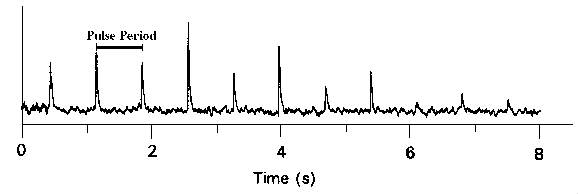
\includegraphics[width=0.5\linewidth]{Immagini/pulsar pulses.png}
    % \caption{}
    \label{fig: pulsi pulsars}
\end{figure}\\
Si noti che il fattore $\gamma$ che compare nel sincrotrone diminuisce la velocità angolare, come se l'elettrone fosse diventato più pesante, o volendo anche a causa della dilatazione temporale.
Tanto più la velocità aumenta, tanto più gli impulsi si spazieranno ($P\propto\gamma$), e si stringeranno (larghezza $\Delta t\propto\gamma^{-2}$).
Il singolo impulso non si risolve temporalmente, per cui è necessario utilizzare la \textbf{Trasformata di Fourier} (FT),
\footnote{
La FT di un "pettine" di delta, caso per $\gamma$ molto grande, è a sua volta un pettine di delta: più sono "rade" nel tempo, più sono "fitte" nelle frequenze.
Al limite i picchi nel tempo sono infinitamente lontani, mentre in frequenze a infinito le delta diventano infinitamente vicine, diventando una cosa perfettamente orizzontale (in realtà non sono delta perfette, e non verrà fuori qualcosa di perfettamente orizzontale per questo).
}
e ciò che si trova nel caso relativistico è che lo spettro tende a diventare lo spettro \textit{continuo} di \textbf{sincrotrone}, come in \textbf{Figura \ref{fig: spettro di sincrotrone}}.
\begin{figure}[h!]
    \centering
    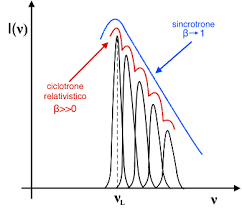
\includegraphics[width=0.4\linewidth]{Immagini/spettro sincrotrone.png}
    \caption{Spettro di emissione caratteristico del sincrotrone.}
    \label{fig: spettro di sincrotrone}
\end{figure}
Da ciclotrone, quando diventa relativistico si trasforma in uno spettro continuo a \textit{legge di potenza}.
Ricapitolando, nelle gap interne prende piede un'emissione su linee di campo poco curvate, nella banda del radio!
Si noti che questa è pur sempre una minima parte dell'emissione totale:
la maggior parte ricade nelle onde a $\sim30Hz$ o nelle gap esterne aperte.
Pure nelle gap interne, questa emissione causata da velocità perpendicolari al campo è la minima parte dell'energia: la maggior parte è comunque lungo il campo. 
Nel complesso, l'emissione coerente in banda radio (temperatura di brillanza di $T\sim10^9K$) è energeticamente irrilevante; tuttavia, è a una frequenza molto maggiore della frequenza di plasma del plerione, e quindi arriva a noi indisturbata, insieme al grosso dell'energia riemessa termicamente dal plerione stesso.


\subsection{Come evolvono nel tempo?}
Partiamo con il generalizzare quanto visto nella \eqref{eq: variazione vel. ang. per emissione di dipolo rotante}:
\begin{equation}
    \dot{\Omega}=-k_n\Omega^n,
    \label{eq: generalizzazione variazione Omega}
\end{equation}
dove con $k_n$ si intende che ci sarà un valore diverso per ogni valore di $n$, detto indice di "\textbf{braking}" (nel caso di dipolo magnetico perfetto, abbiamo visto che $n=3$ e $k_3=\frac{2}{3c^3}\frac{\mu^2}{I}$).
Sperimentalmente, si trova che $n$ è decisamente diverso da $3$, anche di un fattore $10$, ma non ne vedremo i motivi in questo contesto: noi considereremo come se $n=3$.
Dunque, si può trovare
\begin{equation}
    \frac{d\Omega}{\Omega^n}=-k_ndt \xrightarrow{} -\left[ \frac{1}{n-1}\frac{1}{\Omega^{n-1}} \right]_{\Omega_i}^{\Omega_f} = -k_n(t_f-\not {t_i}),
\end{equation}
dove sto ponendo $t_i =0 $, per trovare infine
\begin{equation}
    \frac{1}{\Omega_f^{n-1}} - \frac{1}{\Omega_i^{n-1}}= (n-1)k_nt_f\hspace{1mm}.
    \label{eq: evoluzione temporale velocità angolare}
\end{equation}

\subsubsection{Tempo di vita e tempo di spin-down}
Dalla \eqref{eq: evoluzione temporale velocità angolare} si può notare che per $t_f\xrightarrow{}0$, torna $0=0$, mentre per $t_f\xrightarrow{}\infty$, $\Omega_i>>\Omega_f$:
se passasse abbastanza tempo, dunque, si avrebbe
\begin{align}
    &\frac{1}{\Omega_f^{n-1}} = \frac{\Omega_f}{\Omega_f^n}\simeq(n-1)k_nt_f\\
    &\xrightarrow{} -\frac{\Omega_f}{\dot{\Omega}_f} \simeq (n-1)t_f\\
    &\xrightarrow{} \frac{P}{\dot{P}} \simeq (n-1)t \hspace{1mm}, 
\end{align}
ricordando la \eqref{eq: generalizzazione variazione Omega}, che riscriviamo come:
\begin{equation}
    \tau_{age}\sim \frac{P}{\dot{P}}\frac{1}{(n-1)}\hspace{1mm}.
    \label{eq: tempo di vita ns}
\end{equation}

Si noti che
\begin{align}
    &\frac{1}{\Omega^{n-1}}= \left(\frac{P}{2\pi}\right)^{n-1} \simeq (n-1)k_nt \\
    &\xrightarrow{} P\simeq\Lambda t^{\frac{1}{n-1}},
    \label{eq: periodo radice n-1 esima di t}
\end{align}
che per $n=3$ significa che il periodo va come la radice quadrata del tempo.
Ora, questo risultato lo abbiamo ottenuto assumendo che il tempo iniziale fosse pari a $0$: finché il tempo iniziale è molto piccolo, il tempo che valuto con la \eqref{eq: tempo di vita ns} è sufficientemente corretto, perché la radice è una funzione che cresce molto lentamente, e quindi il nostro risultato dipende molto poco dal valore iniziale.
Nel caso della Crab nebula, il tempo di vita viene pari a $\tau\sim3,3\cdot10^{10}s \sim 1000yr$\footnote{Astronomi cinesi nel 1054 a.c. osservarono in effetti una nuova stella che durò circa un mese, in grado anche in pieno giorno di proiettare una seconda ombra!
In questo caso, tuttavia, aver azzeccato il tempo di vita è stata una botta di fortuna. 
Infatti tecnicamente nel corso di mille anni il campo magnetico non è certamente costante  come abbiamo assunto, soprattutto per pulsar vecchie; inoltre, pulsar vecchie diventano meno regolari. 
Tutto sommato, in generale il fatto che $n=3$ ce lo possiamo scordare.
Tuttavia, la fortuna è stata proprio che la Crab è una pulsar giovane, e quindi le assunzioni possono ancora valere.}. 
Prendendo la \eqref{eq: tempo di vita ns} per $n=3$, si vede che 
\begin{equation}
    \tau_{age}\leq \frac{P}{2\dot{P}} = \tau_{sd},
\end{equation}
dove abbiamo definito $\tau_{sd}$, la \textbf{spin-down age}.
Si tratta di un limite superiore, che dà una stima di quanto ha vissuto la pulsar.
Ricordiamo che nella \eqref{eq: periodo radice n-1 esima di t} la costante $\Lambda$ non è necessariamente davvero costante: $k$ potrebbe non essere costante in generale, e pure $\mu$ può dipendere dal tempo (nel qual caso andrebbe integrato).
Le assunzioni che abbiamo fatto finora sono due:
\begin{itemize}
    \item la pulsar è partita con un periodo $P_0$ molto più piccolo, dunque trascurabile;
    \item $\mu=cost.$, che è ragionevole se la supernova è avvenuta da poco. Più il tempo di spin-down è grande, più mi aspetto che questa ipotesi decada.
\end{itemize}
Per pulsar mediamente giovani, i due tempi grossomodo appattano.

\subsubsection{Tecnica dinamica}
% Per verificare la $\tau_{age}$.
I vecchi resti di supernova (SNR) assumono una forma di shell, e da modelli che descrivono la velocità di espansione della nube è possibile farsi una prima idea di quanto \textit{questa} sia vecchia.
La maggior parte dei SNR, tuttavia, non presentano la pulsar!
Infatti, nell'esplosione la stella di neutroni parte con una certa velocità a causa del \textbf{natal kick}: le parti esterne esplodono simmetricamente, mentre la NS parte via a velocità di centinaia di km/s!!
Dopo un po' di tempo capita che, in centinaia di migliaia di anni, la NS sia andata anche molto lontana.
In alcuni casi l'associazione nube-pulsar è ovvia (vedi \textbf{bullet nebula}), e si può stimare anche la \textbf{kick velocity}: $v_{kick}$.

\section{Diagramma BP}
I parametri sperimentali sono $\nu,\dot{\nu},P,\dot{P}$, e il diagramma che vedremo è una versione non recente, che usa la relazione fra campo magnetico e periodo, e rappresenta il logaritmo del primo in funzione del logaritmo del secondo.
In questa versione, le linee di campo magnetico costante sono orizzontali, mentre quelle di periodo costante sono verticali.
\begin{figure}[h!]
    \centering
    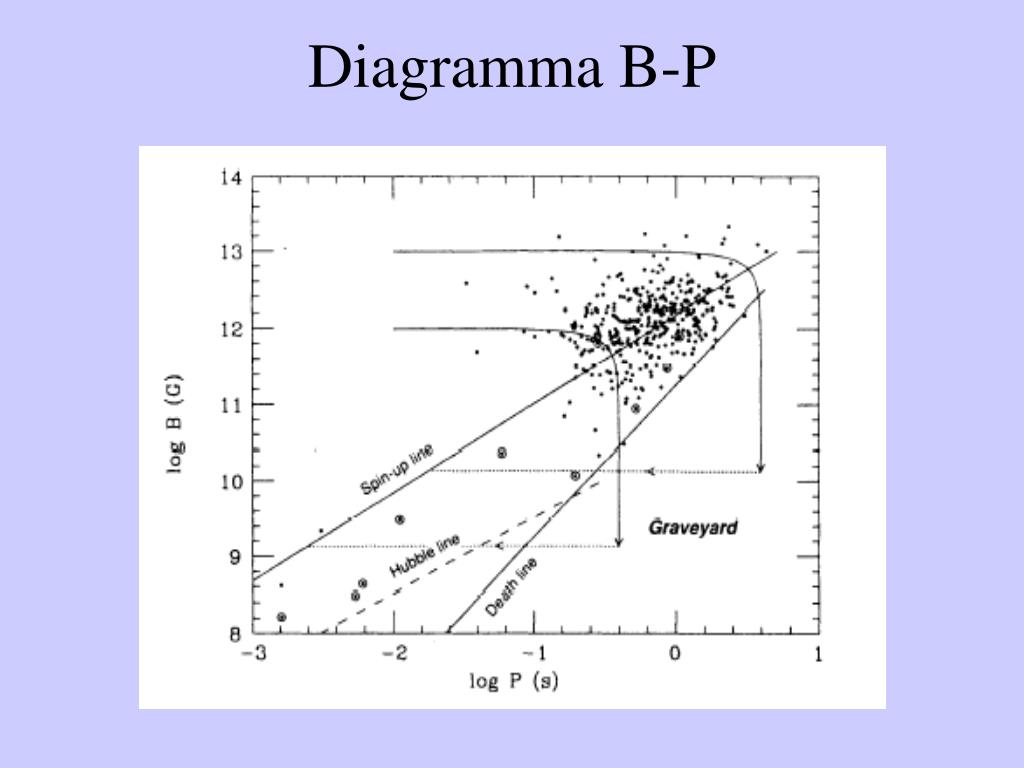
\includegraphics[width=0.7\linewidth]{Immagini/diagramma-b-p-l.jpg}
    %\caption{Caption}
    \label{fig: diagramma BP}
    \caption{Diagramma che mostra l'evoluzione delle NS in termini di relazione campo magnetico - periodo.}
\end{figure}

\subsection{Linee importanti}
Nel diagramma ci sono diverse linee che descrivono i moti delle NS al suo interno, e ora vedremo come sono state dedotte le più importanti.
\subsubsection{Hubble line}
Ora, si noti che unendo la \eqref{eq: B in funzione di PPdot} con la \eqref{eq: tempo di vita ns}, si trova che 
\begin{equation}
    B\propto \frac{P}{\sqrt{\tau_{age}}}. 
\end{equation}
Ricordando la legge di Hubble $v=Hr$, si può definire un tempo di vita limite a ordine zero $t_{univ}=1/H$, che faccia da limite superiore al $\tau_{age}$: inserendo questo valore:
\begin{align}
    &\frac{P}{2\dot{P}}=\frac{P^2}{2P\dot{P}}=H_0^{-1}\\
    &\xrightarrow{} \left(\frac{P}{B}\right)^2=\frac{2}{H_0\cdot3,2\cdot10^{19}}\\
    &\xrightarrow{}B=W_{H_0}P,
\end{align}
dove abbiamo inserito il valore della costante di proporzionalità in $B=cost.\sqrt{P\dot{P}}$ in \eqref{eq: B in funzione di PPdot}, e riscrivendola infine diventa
\begin{equation}
    \log B = \log W_{H_0}+\log P.
    \label{eq: equazione hubble line}
\end{equation}
Quella appena descritta, è una linea nel diagramma dalla pendenza circa pari a $1$, oltre la quale non possono andare, che prende il nome di \textbf{Hubble line} (HL).
Immaginiamo una pulsar con un $B$ costante, che muove su una linea quindi orizzontale con un periodo che cambia come $P=\sqrt{P_0^2 + kt} $, quindi più velocemente all'inizio e andando poi a rallentare;mano a mano che rallenta, la pulsar arriverà quasi a toccare eventualmente la HL, che concettualmente non può raggiungere: le pulsar si accumuleranno in prossimità di essa.

\subsubsection{Death line}
Se è vero che il rallentamento del periodo è dovuto fondamentalmente alle onde a $\sim30Hz$, ricordiamo però che l'emissione radio che vediamo dalle pulsar è invece dovuta all'emissione di curvatura delle cariche, che si formano a coppie laddove l'energia dell'emissione delle cariche precedenti fosse stata $\sim 1MeV$.
Al di sotto di questa soglia, l'emissione radio non avviene più, si spegne.
La condizione da imporre in questo caso è
\begin{equation}
    \frac{2}{3c^3}\mu^2\Omega^4 = \frac{2}{3c^3}B_{eq}^2R_{NS}^6\left(\frac{2\pi}{P}\right)^4\geq L_{soglia},
\end{equation}
che si riscrive come
\begin{equation}
    B_{eq}\geq cost.P^2 \xrightarrow{} \log B_{eq} \geq \log K+ 2\log P,
\end{equation}
che è una retta nel diagramma, con pendenza peri a $2$, oltre la quale le pulsar si spengono nell'emissione radio (e quindi come pulsatori periodici), e smettono di essere per noi visibili: da questo, il nome \textbf{Death line}.

\subsubsection{Linee curve}
Per capire cosa sono le linee curve che appaiono nella \textbf{Figura \ref{fig: diagramma BP}} dobbiamo parlare meglio dei campi magnetici.
Chiaramente, stelle di neutroni come perfetti dipoli non esistono; esistono però le correnti.
Nelle stelle di neutroni, come nei grossi nuclei, ci sono molti più neutroni che protoni, per compensare la repulsione; inoltre, in questo caso è la gravità a tenere i nucleoni legati.
La piccola frazione di protoni che è presente, è caricamente compensata da una piccola quantità di elettroni, con i quali si respingono e distribuiscono come nei conduttori: in superficie (oltre che per altri motivi statistici).
In una struttura cristallina perfetta, l'elettrone è come un'onda piana che disperde a seconda delle proprietà dei cristalli con una velocità costante, senza sentire resistenze; sotto enormi pressioni la materia cristallizza, e quindi mi posso aspettare che in una stella di neutroni la materia formerebbe una struttura cristallina perfetta: sulla superficie di una NS, gli elettroni si muovono liberamente come su un cristallo perfetto, mostrando un comportamento simile a un superconduttore!\footnote{\url{https://en.wikipedia.org/wiki/Cooper_pair} per approfondire.}
Se già in un metallo la resistenza è bassa, nei superconduttori (come nella superficie di una NS) non c'è nessuna resistenza: è come se avessi un enorme solenoide con resistenza pari a $0$, un'unica fascia di corrente di cariche dentro la quale il campo è dritto, e fuori è quello di un dipolo.
In realtà, più che un unico cristallo perfetto la NS è come un mosaico di cristalli orientati in direzioni casuali.
Questi difetti reticolari fanno sì che una piccola, ma non nulla, resistività residua ci sia (stiamo comunque parlando di tempi scala di decadimento dell'ordine di $10^6-10^9yr$!).
Inoltre, più aumenta la pressione, più il comportamento è perfettamente cristallino\footnote{Le nane bianche da fuori apparirebbero come delle palle di metallo, estremamente lisce (a causa dell'enorme gravità che appiattisce le asperità: con la gravità alla superficie di una WD, le asperità riscalate corrispondono ad asperità delle dimensioni di un atomo sulla terra), di densità di $\sim 1 \frac{Ton}{cm^3}$: come dei geoidi di mercurio.
Attorno a questo geoide, il carbonio estremamente compresso cristallizzerebbe vicinissimo alla superficie, formando uno strato di diamante sottilissimo (più in profondità la pressione sarebbe troppa per essere sorretta dalla struttura del diamante).
Sicuramente, a causa dell'enorme gradiente di pressione, appena sotto la superficie gli elettroni sono già praticamente liberi, in quanto la pressione che sostiene la stella è la degenerazione neutronica.
Ricordiamo inoltre, che alla superficie la pressione è nulla, per cui in superficie uno strato di elementi come elio, o carbonio può ancora resistere (e quindi fondere): quando sono più a fondo sono troppo compressi per resistere, e avviene la neutronizzazione.}: al centro diventano anche più perfetti.\vspace{3mm}\\
Ora, sapendo che $R_{NS}\sim \frac{R_{WD}}{1000} $, e ovviamente $S\propto R^2 $, allora il campo aumenterà, al diminuire del raggio nel collasso, come $R^{-2}$: $B_{NS}\propto 10^6B_{WD} \sim 10^{12}G$.\footnote{Ricordiamo che quando una nana bianca finisce, dopo una serie di cicli, per avere un nucleo di ferro, le uniche reazioni che possono continuare ad avvenire sono endogene, cioè assorbono energia anziché rilasciarne, accelerando il collasso.
Finché le particelle sono non relativistiche, la nana bianca resta sorretta dalla pressione di degenerazione degli elettroni; quando le pressioni però rendono le parti interne relativistiche (masse oltre $1,44M_{\odot}$), la pressione di degenerazione degli elettroni non regge più e interviene quella dei neutroni.}
Il flusso magnetico $\phi_B=BA $ si conserva, quindi se la superficie $A$ cresce, il campo deve decrescere, e viceversa.
Questo perché se ci sono campi ci sono correnti elettriche, e la sorta di "congelamento del campo" che abbiamo descritto è dovuta al fatto che le correnti elettriche devono continuare ad esserci. 
Infatti, mentre sulla superficie di una NS i protoni e i neutroni sono attaccati a distanze di alcuni fermi, gli elettroni sono liberi di muoversi, e formano una specie di fascia cilindrica di corrente, in cui la resistenza è talmente bassa che anche senza un generatore le cariche continueranno a scorrere: esattamente come le cariche in un circuito chiuso saranno rallentate dalla resistività del circuito stesso, e la corrente diminuirà quindi esponenzialmente.
Ora, se scaldo la superficie esterna, la conduttività peggiora, per cui alla superficie mi aspetto correnti che decadono esponenzialmente alla superficie:
\begin{equation}
    I(t)=I_0e^{-\frac{t}{\tau}} \xrightarrow{} B=B_0e^{-\frac{t}{\tau}},
    \label{eq: decadimento esponenziale}
\end{equation}
dove $\tau$ è il tempo di decadimento della corrente.
Anche se ci sono correnti sub-crostali molto intense, su conduttori estremamente buoni, è inevitabile che si dissipino e che i campi magnetici ne risentano.

\subsection{Altre considerazioni sul diagramma}
\subsubsection{$\mathbf{\Omega(t)}$, $\mathbf{B(t)}$ e comportamenti asintotici grafico BP}
Ora quello che sappiamo è riassunto come segue
\begin{equation}
    \left\{ 
    \begin{array}{rcl}
    \dot{\Omega}  = & -k_{n=3}\Omega^3  =  -WB^2\Omega^3 & (equazione\hspace{2mm}differenziale)\\
    B  = & B_0e^{-\frac{t}{\tau}} & (equazione\hspace{1mm}integrale),
    \end{array} % correggi impostazione
    \right.
    \label{eq: versione differenziale e integrale a confronto}
\end{equation}
da cui si può ottenere 
\begin{align}
    &\frac{d\Omega}{dt} = -WB_0^2e^{-\frac{2t}{\tau}}\Omega^3\xrightarrow{} \frac{d\Omega}{\Omega^3}\propto -e^{-\frac{2t}{\tau}}dt\notag \\
    &e\hspace{1mm}integrando:\notag\\
    &-\frac{1}{2}\left[ \frac{1}{\Omega_f^2} - \frac{1}{\Omega_i^2} \right] = k\frac{\tau}{2}\left[ e^{-\frac{2t_f}{\tau}} - 1 \right],
\end{align}
da cui si ottiene una $\Omega(t)$.
Dunque inizialmente, per $t<<\tau_B$, con $\tau_B$ il tempo di decadimento dei campi magnetici, il campo sarà $B\sim B_0e^0 \sim B_0 = cost.$, e la linea sarà orizzontale.
Quando invece mi avvicino alla HL, per $t\xrightarrow{}\tau_{Hubble}$, è il periodo ad essere costante, e la linea sarà verticale.
Questi sono i due comportamenti asintotici delle linee curve spiegati: a mano a mano che il campo deteriora, il suo valore diminuirà, e ci si avvicina a tempi per cui il periodo si stabilizza (dalla prima delle \ref{eq: versione differenziale e integrale a confronto}: se $B \xrightarrow{} 0$, allora la variazione della frequenza va a 0).
La curva si spiega così, notando che $\tau_B \sim 10^8yr$ mentre $\tau_H \sim 10^{10}yr$. 
Se $\tau_B$ fosse maggiore di $\tau_H$, nel grafico avrei solo linee orizzontali senza curve; viceversa, se fosse molto molto minore, vedrei solo curve verticali.
Le linee che vedo non sono esattamente orizzontali né perfettamente verticali, perché il campo e il periodo variano sempre un po'.
Il campo però, può cambiare anche per fattori esterni come una variazione della temperatura: i fononi, scaldando, aumentano le interazioni con gli elettroni, rallentandoli.
Inizialmente, la crosta è calda dopo la supernova, per cui mi aspetterei un raffreddamento iniziale con conseguente variazione del campo magnetico.
Tuttavia, le stelle che vedo sono concentrate vicino alle curve, come si vede in \textbf{Figura \ref{fig: diagramma BP}}, e \textit{non posso sapere se sono arrivate lì con un campo costante, o con un campo che ha raggiunto quel valore dopo essere decaduto}; se non ci fosse la DL, potrei vedere come proseguono le stelle nel diagramma, e capirei se arrivano da un decadimento di B oppure no.

\subsubsection{Sull'interno delle stelle di neutroni (APPENDICE?)}
Come sappiamo, protoni e neutroni sono delle combinazioni di quark \textit{up} e quark \textit{down} in tripletti.
Quando in questi tripletti compare anche un quark \textit{strange}, si possono inoltre formare "super neutroni", che sono più massivi di quelli normali.
Si può ipotizzare un tipo di materia in cui le cose però non sono organizzate in maniera ordinata in questo modo a tripletti, ma piuttosto in "righe" di quark talmente compressi fra loro da non essere riconoscibilmente organizzati in gruppi separati, persi in un'individualità, una sorta di "pappa" di quark di questi tre tipi (up, down e strange): questa configurazione prende il nome di \textbf{Strange Quark Matter} (\textbf{sqm}).\footnote{Finché ho barioni, tripletti distinti, ho particelle $\sim$ identiche, e devo piazzarli a livelli.
Nella sqm invece, avrei una pappa autolegata, con una composizione media $\sim uds$ che non si aggrega in singole e individuali particelle.}
Questa configurazione, è come se perdesse la pressione di degenerazione che normalmente fa salire di energia man mano che aggiungo barioni.
Nei nuclei, è la \textit{forza forte}, mediata da scambi di pioni, che permette al nucleo di restare coeso e ai barioni di legarsi, e se venisse a mancare i nuclei esploderebbero.
Più sono grossi i nuclei maggiore deve essere questa forza per contenerli.
Nella sqm, invece, occorrerebbe una forza legante a long range.
La stella di neutroni, a causa dell'enorme pressione di degenerazione, senza la gravità esploderebbe: ciò a meno che la materia non sia \textit{self bound}, ovvero \textit{autolegata}, come nel caso della sqm \footnote{Tutta la materia che conosciamo è auto legata: non è la gravità a tenerla assieme, ma legami elettrici fra gli orbitali atomici.
D'altro canto, materia legata gravitazionalmente come ad esempio le nane bianche, sono estremamente dense per via della gravità, e in assenza di questa un "cucchiaino" di WD portato qui sulla terra si espanderebbe immensamente, non essendo più trattenuta in quello stato così denso da niente}.
Essendo esente da pressione di degenerazione, una materia simile sarebbe lo stato (auto) legato più stabile della materia.
La trasformazione in sqm si verificherebbe nel centro di normali NS con $\rho \sim 10\rho_{nuc}$, nelle quali il centro conterrebbe una fase per la quale il politropo cambia.
La soluzione generale ovviamente poi sarebbe un collage molto complicato di soluzioni diverse.

\subsubsection{Posizione NS nel diagramma BP}
Perché nel diagramma non si vedono stelle con piccoli periodi e grandi campi magnetici?
Come si vede dalla \eqref{eq: variazione vel. ang. per emissione di dipolo rotante} per grandi velocità angolari la variazione è rapidissima: rallentano (e quindi il periodo aumenta) velocemente emettendo un botto.
Mantenendo un campo magnetico alto non posso avere periodi piccolissimi perché evolvono velocissime verso destra: se ne vedessi una vorrebbe dire che è una stella nata "ieri", il che è molto improbabile.
Capita invece di vedere stelle più in basso nel grafico, che nascono con campi magnetici dell'ordine di $\sim 10^8G$.
Tuttavia, le pulsar sono oggetti così estremi che ci si può aspettare che siano più o meno tutte uguali: l'unica vera libertà è la massa, e anche quella non varia così tanto.
Per il resto, c'è solo $n$.
Chiaramente, esistono diversi modelli, ma una volta capito qual è quello giusto, più o meno sarà quello che le descrive tutte.
Questo ci porta a credere che le NS con campi di $\sim10^8G$ non siano davvero nate così diverse, ma che siano così come le osserviamo per via di scenari legati all'accrescimento.

\subsubsection{Scenario del riciclaggio}
L'idea è la seguente: stelle che oltrepassano la DL e smettono di essere visibili seguono un percorso nel quale scendono verso il basso (dove si trova il "graveyard", o "cimitero" nella \textbf{Figura \ref{fig: diagramma BP}}) per poi, per motivi che vedremo, in certi casi riaccelerare e tornare verso sinistra prima della DL in "basso".
Ora, se a ordine 0 assumiamo la densità delle NS come costante, allora sapendo che
\begin{equation}
    L_{NS} = I_{NS}\Omega = \frac{2}{5}MR^2\Omega,
\end{equation}
accrescendo materia con momento angolare aumenteranno anche il momento di inerzia e la velocità angolare: spostandosi verso sinistra (all'aumentare di $\Omega$) aumenterà la luminosità!
La materia in orbita Kepleriana nel disco ha un momento angolare per unità di massa $l=rv_k$, dove $v_k = \Omega_kr $ e $\Omega_k^2 = \frac{GM_{tot}}{r^3} $, per CM coincidente con l'oggetto compatto, la cui massa è molto maggiore della massa che sta cadendo.
Quindi: $v_k=\sqrt{\frac{GM}{r^3}}r $ per cui si trova che $l=\sqrt{GMr}$.
Dato che abbiamo un $\dot{M}$, possiamo chiederci il valore del tasso di variazione del momento angolare della stella di neutroni:
\begin{equation}
    \frac{\dot{l}}{l} = \frac{1}{2}\frac{\dot{M}}{M} \xrightarrow{} \dot{l} = \frac{1}{2}\frac{\dot{M}}{M}\sqrt{GMr}.
\end{equation}
Mettendo qualche numero, si trovano valori dell'ordine $\frac{\dot{l}}{l}\sim 10^{-17}$: in prima battuta posso trascurare la variazione di momento angolare dovuta all'aumento della massa della NS.
Concettualmente il tasso a cui la NS acquista materia su un tempo scala istantaneo è una quantità fissata.
\begin{equation}
    \dot{L}=l\dot{M}\xrightarrow{} \frac{\dot{L}}{L} = \frac{l\dot{M}}{I\Omega} = \frac{\dot{I}}{I} + \frac{\dot{\Omega}}{\Omega},
\end{equation}
per cui infine 
\begin{equation}
     l\dot{M} = \dot{I}\Omega + I \dot{\Omega} .
    \label{eq: l Mdot}
\end{equation}
Ora, la stella di neutroni è un politropo di indice $3/2$, ma in primissima battuta $\rho_{NS}\sim cost.$, e si può tenere conto della NON costanza con un termine $\alpha$ dell'ordine dell'unità: $I = \alpha \frac{2}{5}MR^2$.
Facciamo l'approssimazione che, aumentando la massa, l'indice politropico resti circa costante, e quindi $\alpha\sim cost.$; allora si ha che 
\begin{equation}
    \frac{\dot{I}}{I} = \frac{\dot{M}}{M} + \frac{2\dot{R}}{R}.
\end{equation}
Per una NS, $R\propto M^\beta$ dove, per indice politropico di $3/2$, $\beta = -1/3$, e quindi $\frac{\dot{R}}{R} = \beta\frac{\dot{M}}{M}$,  per cui 
\begin{equation}
    \frac{\dot{I}}{I} = \frac{\dot{M}}{M}\left[1+2\beta \right].
    \label{eq: Idot su I}
\end{equation}
Dalla \eqref{eq: l Mdot}, sostituendo $I = \alpha\frac{2}{5}MR^2$ e dividendo ambo i lati per $I$, si ottiene
\begin{equation}
    \frac{\dot{I}\Omega}{I} + \dot{\Omega} =\frac{l\dot{M}}{\alpha\frac{2}{5}MR^2},
\end{equation}
e quindi inserendo la \eqref{eq: Idot su I}
\begin{align}
    \dot{\Omega} = \frac{l\dot{M}}{\alpha\frac{2}{5}MR^2} - \frac{\dot{M}}{M}(1+2\beta)\Omega \notag\\
    \xrightarrow{} \frac{\dot{\Omega}}{\Omega} = \frac{\dot{M}}{M}\left[ \frac{5l}{2\alpha R^2\Omega}-1-2\beta \right]\notag\\
     =  \frac{\dot{M}}{M}\left[ \frac{5\sqrt{GMr}}{2\alpha R^2\Omega}-1-2\beta \right],
     \label{eq: Omega su Omega dot}
\end{align}
dove $r$ è il raggio da cui viene agganciata la materia.
Si nota quindi che, se $\Omega>0$, come $\dot{\Omega}$ aumenta, aumenta la velocità angolare e quindi diminuisce il periodo.
Questo permette alla NS di "tornare in vita", cioè tornare visibile e quindi entro la DL.
Ricordiamo che il valore di $\beta$ è pari a $-\frac{1}{3}$ per stelle puramente di neutroni, $0$ laddove il raggio non dipende dalla massa, e $\frac{1}{3}$ per densità costante (sqm).
Noi in generale assumeremo che $1+2\beta \sim 1$.
Considerando che $\frac{\sqrt{GMr}}{R^2\Omega}\sim10^{2-3}$, il primo termine nella \eqref{eq: Omega su Omega dot} rende la variazione della frequenza positiva: l'accrescimento determina così un processo di \textbf{SPIN UP}.
In questa stima, abbiamo considerato un $r\sim10^{10}cm$; prendiamo il caso limite in cui il raggio della materia che cade sia dell'ordine del raggio della NS, $r\sim R_{NS} \sim 10^6 $cm: il primo termine scende di un fattore $10^2$, diventando confrontabile con il secondo!

\section{Raggi importanti}

\subsection{Descrizione energetica}
Occorre quindi determinare meglio $r$: sui BH si usa l'ISCO, mentre nelle NS occorre tenere conto del campo magnetico.
Una descrizione in termini energetici è molto più semplice rispetto a una descrizione in termini di forze, per cui descriveremo attraverso i fluidi e le pressioni i comportamenti del disco
\footnote{
Si noti infatti che la pressione dimensionalmente è una densità di energia: $[P] = \frac{F}{A} = \frac{F}{r^2} = \frac{Fr}{r^3} = \frac{Energia}{Volume} $. Si può pensare alla pressione come a una forma di energia immagazzinata.
}.
Daremo una descrizione per la quale se la densità di energia di A è maggiore della densità di energia di B, la materia si muove secondo le leggi del sistema A.
Nel nostro caso, il confronto avverrà fra la materia in orbita Kepleriana del disco, con densità di energia $\epsilon_k$, ed il "fluido magnetico" di densità energetica $\epsilon_\mu$:
\begin{itemize}
    \item se $\epsilon_k>\epsilon_\mu$ la materia segue le leggi kepleriane, come se il campo magnetico non ci fosse;
    \item se $\epsilon_k<\epsilon_\mu$, la materia obbedirà alle forze di Lorentz, che costringono la materia a muoversi lungo le linee di campo;
    \item se $\epsilon_k = \epsilon_\mu$ e risolvo per $r$, trovo il valore del raggio entro cui domina una, e oltre il quale domina l'altra, detto \textbf{raggio magnetosferico}.
\end{itemize}

\subsubsection{Caduta radiale}
Nel caso estremo di momento angolare nullo, trascurando le componenti angolari avremo una densità di energia di caduta libera e quella magnetica, che uguaglieremo:
\begin{equation}
    \epsilon_\mu = \frac{B^2(r)}{8\pi} = \frac{\mu^2}{8\pi}r^{-6}\sim \frac{1}{2}\rho v_{ff}^2 = \frac{1}{2}\rho \frac{2GM}{r} = \epsilon_{ff}.
    \label{eq: uguaglianza densità energie}
\end{equation}
Ora, se la materia cade radialmente da ogni direzione, varrà un'equazione di \textbf{continuità}:
\begin{equation}
    \rho(r)v_{ff}(r)4\pi r^2 = cost. = \dot{M}
\end{equation}
Infatti, esattamente come in una tubatura ad essere costante dev'essere la quantità di liquido che passa per unità di tempo, anche al variare della sezione, anche qui dovrà valere lo stesso per la massa che cade.
Segue quindi che
\begin{equation}
    \rho = \frac{\dot{M}}{4\pi\sqrt{2GM}}r^{-3/2},
\end{equation}
e sostituendo in \eqref{eq: uguaglianza densità energie}:
\begin{align}
    \frac{\mu^2}{8\pi}r^{-6} &= \frac{\dot{M}}{4\pi\sqrt{GMr}}r^{-3/2}\frac{GM}{r}\notag\\
    r^{7/2} &= \frac{\mu^2\sqrt{2}}{2\dot{M}\sqrt{GM}}\notag,
\end{align}
da cui si ottiene il \textbf{Raggio di Alfvén}:
\begin{equation}
    \boxed{R_A = \frac{1}{\sqrt{2}}\mu^{4/7}\left(\frac{GM}{2}\right)^{-1/7}\dot{M}^{-2/7}}\hspace{1mm}.
    \label{eq: raggio di Alfvén - radiale}
\end{equation}
Come si vede, più $\mu$ cresce, più cresce il raggio, così come più $\dot{M}$ cresce, più il raggio diminuisce (in quanto aumenta la densità) e più $M_{NS} $ è piccola più il raggio cresce.
Inoltre, sono dipendenze abbastanza deboli: la dipendenza maggiore è, per distacco, quella dal campo magnetico $B$.
Ora, poiché $\mu=R^3B = 10^{18}cm^3\cdot10^8G \sim10^{26} cm^3G$, mentre $\dot{M}\sim10^{-8}M_{\odot}/yr $, è utile riscrivere il raggio di Alfvén come 
\begin{equation}
    R_{A_6} = \mu_{26}^{4/7}m^{-1/7}\dot{m}^{-2/7}_{-8}.
    \label{eq: Alfvén radiale unità comode}
\end{equation}
Tutto questo, ricordiamo, vale nell'ipotesi di accrescimento radiale, che è un caso molto estremo.

\subsection{Descrizione dinamica}
Adesso daremo una descrizione in termini dinamici, quindi di forze, ponendoci sul piano equatoriale.
Nei casi in cui la NS ha una compagna molto più grande, che alimenta la NS più di quanto questa non "digerisca", questo fenomeno avviene in maniera circa sferica, e le situazioni che si presentano sono come quelle descritte in seguito.

\subsubsection{Campi indotti e forze - accrescimento sferico}
Si consideri $1cm^2$ di superficie del disco perpendicolare al piano equatoriale: su questo si formerà una corrente superficiale, in quanto le cariche del plasma muoveranno radialmente lungo il disco.
Attraverso la superficie considerata, è come se passasse la corrente che si genera in un conduttore, però si muovono anche cariche positive (plasma).
La carica che muove radialmente, a causa della presenza di un campo magnetico della NS stessa, che come il campo di un dipolo sarà perpendicolare al piano equatoriale, sentirà una forza di Lorentz che la spingerà nella direzione, sul piano equatoriale, perpendicolare alla direzione radiale:
\begin{figure}[h!]
    \centering
    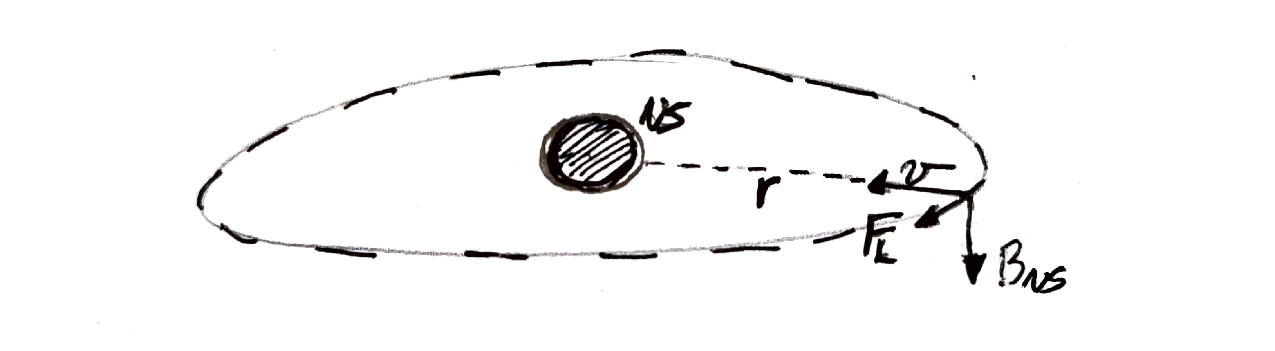
\includegraphics[width=0.65\linewidth]{Immagini/carica in orbita fase 2.pdf}
    % \caption{Caption}
    \label{fig: carica in orbita fase 1}
\end{figure}\\
La carica si metterà così in movimento, al suo raggio $r$, lungo una circonferenza nel disco: questo genererà un nuovo campo magnetico, che entro $r$ si sommerà positivamente con quello della NS, mentre fuori da $r$, avendo direzione opposta, vi si opporrà:
abbiamo così una situazione in cui entro questo raggio il campo raddoppia, mentre al di fuori si annulla!
\begin{figure}[h!]
    \centering
    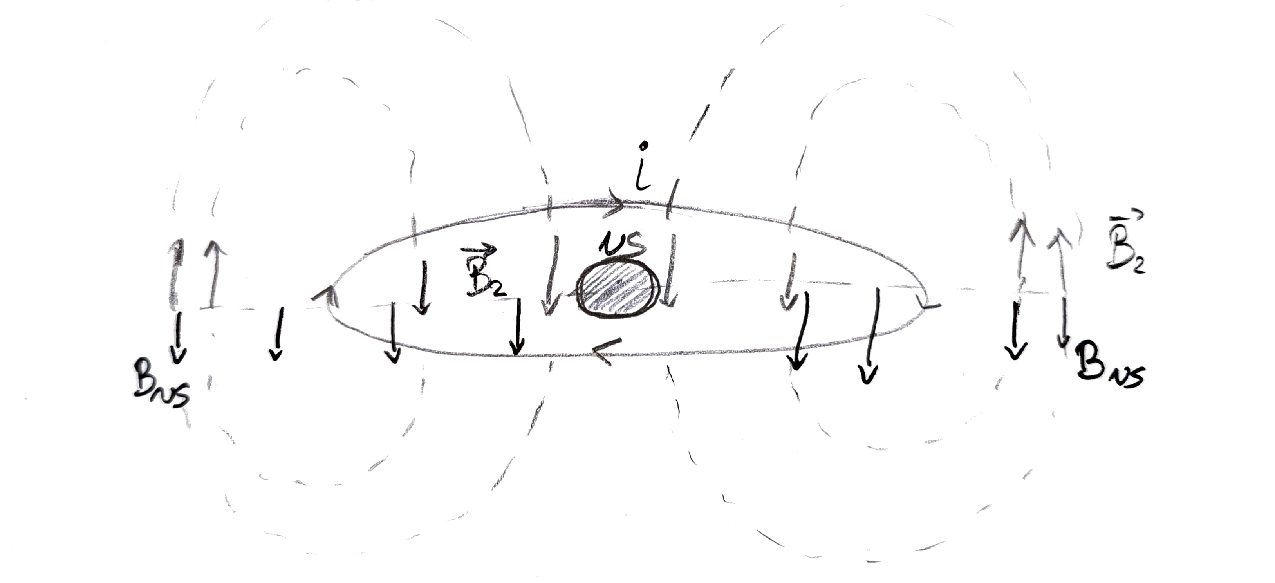
\includegraphics[width=0.65\linewidth]{Immagini/carica in orbita fase 1 .pdf}
    % \caption{Caption}
    \label{fig: carica in orbita fase 2}
\end{figure}\\
Ora che le cariche si muovono circolarmente, nella regione interna dove c'è un campo verso il basso si genererà una forza su di esse verso l'esterno, a contrastare l'effetto della forza di gravità!
\begin{figure}[h!]
    \centering
    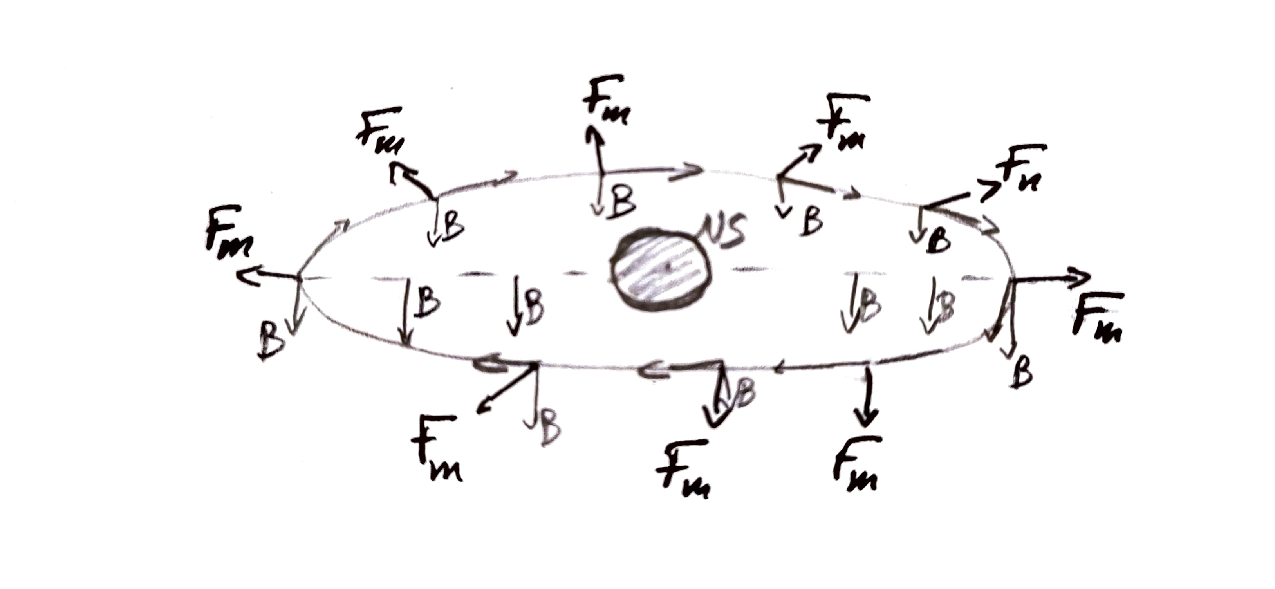
\includegraphics[width=0.65\linewidth]{Immagini/carica in orbita fase 3.pdf}
    % \caption{Caption}
    \label{fig: carica in orbita fase 3}
\end{figure}
Queste due forze saranno uguali, come trovato nella trattazione energetica, a una distanza, che prende il nome di \textbf{raggio magnetosferico} $\mathbf{R_m}$, che sul piano equatoriale sarà proprio uguale al raggio di Alfvén. 
In pratica, si forma una superficie a forma di mela, con due cuspidi ai poli magnetici (qui il raggio è $R_m\sim\frac{1}{2}R_A $), sulla quale le due forze si bilanciano perfettamente.
Si noti che per una NS con un campo dell'ordine dei $10^{12}G$, il $R_A\sim10^8cm \sim10^2R_{NS} $: se tutta la materia si ferma a quella distanza, allora non accresce più per via di questa forza di Lorentz verso fuori?
Se la materia si accumula, si genera una pressione dovuta al moto ordinato di questo fluido che spinge: la \textbf{pressione di ariete}.
Insomma, la materia dovrebbe in effetti comprimersi.
In realtà, la materia in qualche modo riesce a passare grazie alle \textbf{instabilità di Rayleigh-Taylor}, o \textbf{instabilità di scambio}: si tratta di un'instabilità che intercorre fra due fluidi che è presente ogni volta che un fluido più denso si trova sopra un fluido meno denso, e per l'appunto si scambiano fra loro.
\begin{figure}[h!]
    \centering
    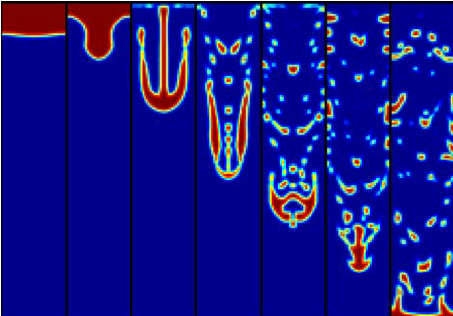
\includegraphics[width=0.4\linewidth]{Immagini/RT_instability.png}
    %\caption{Caption}
    \label{fig: R-T instability}
\end{figure}\\
Oltre alla pressione di ariete, quindi, interviene anche la spinta di Archimede, visto che all'accumularsi della materia, a quel raggio si crea un fluido sempre più denso e compresso.
La materia, come nelle lava-lamp, facendosi strada resta schiacciata e permette all'accrescimento di iniziare in questo modo.
Questo fa sì che ci sia produzione di raggi X, che scalderanno la materia all'esterno favorendo ulteriormente le instabilità di scambio.
Nelle cuspidi questa illuminazione è anche più efficace, cosicché l'accrescimento diventi ancora più forte ai poli del campo magnetico.
Si creano così le chiazze ai poli che, nelle Ns che ruotano, si mostrano a noi a intermittenza nell'X, da cui il nome di "\textbf{pulsatori X}
".
\subsubsection{Accrescimento da disco}
Nel caso in cui l'accrescimento avvenga dal disco, questo va a comprimere, tagliare come una lama il campo magnetico (sempre per il gioco di forze descritto).
Il raggio magnetosferico in questo caso sarà dato da $R_m\sim\phi R_A$, con $\phi\leq1$; i conti sono molto complicati\footnote{Forse il conto esplicito si trova in \cite{Hayakawa}}, e $\phi$ dipende da $M, \dot{M},\alpha,\dots$ molto debolmente.
Senza dover fare i conti si capisce che debba avere valori inferiori all'unità, perché nell'accrescimento radiale la densità del disco è molto elevata ed entrerà di più che nel caso sferico nel quale si è ottenuto $R_A$ ($\rho_{acc_{disco}}\sim100\rho_{acc_{sferico}} $).
% A causa della legge di Lenz, come abbiamo visto, i dischi sono diamagnetici
Quindi, abbiamo detto che all'interno del raggio magnetosferico la materia è dominata dal campo, e sarà costretta  muoversi lungo le sue linee curve di dipolo. 

\subsubsection{Effetto elica}
Se la materia si aggancia alla linea di campo, che si muoverà a $v = \Omega_{NS}R_m $, sentirà una forza centrifuga pari a 
\begin{equation}
    F_c = m\Omega^2_{NS}R_m,
\end{equation}
opposta a $F_g = \frac{GMm}{R_m^2}$.
Uguagliando queste due forze, ricavo quindi il \textbf{Raggio di co-rotazione}:
\begin{equation}
    R_{CO}=\left( \frac{GM}{\Omega_{NS}} \right)^{1/3},
    \label{eq: raggio di corotazione}
\end{equation}
dove ovviamente $\Omega_{NS} $ è la velocità Kepleriana.
Cioè quando il campo si porta dietro la materia, al raggio di co-rotazione la forza centrifuga compensa la gravità negando il moto radiale, e mette così in orbita la materia!
Al raggio di co-rotazione, la velocità angolare Kepleriana della materia è uguale alla velocità angolare della NS; se mi allontano di più aumenta la forza centrifuga, che supera così la gravità scagliando verso fuori la materia (\textbf{effetto elica}, o \textbf{effetto propeller}), mentre se mi avvicino di più, viceversa, la forza di gravità vince e la materia cade verso la NS.\footnote{Si noti che il raggio di co-rotazione è un punto molto instabile: $F_c\propto \Omega r$ e $F_g\propto \frac{GM}{r^2} $, per cui mi aspetto che l'accrescimento prima o poi avvenga; inoltre, un raggio preciso così definito ovviamente non esiste, è solo una nostra descrizione.}
In altre parole:
\begin{itemize}
    \item se $R_m>R_{CO}$: effetto elica, accretion centrifugally inhibited;
    \item se $R_m<R_{CO}$: c'è accrescimento. 
\end{itemize}

\subsection{Confronto fra i raggi}
Ricapitolando, i raggi importanti che abbiamo visto sono quindi i seguenti:
\begin{equation}
\left\{
    \begin{array}{l}
       R_m =   \phi R_A  \\
       R_A = (2GM)^{-1/7}\dot{M}^{-2/7}\mu^{4/7} \longleftrightarrow R_{A_6} = \mu^{4/7}_{26}m^{-1/7}\dot{m}_{-8}^{-2/7}  \\
        R_{LC} =  \frac{c}{\Omega_{NS}} \simeq 5P_{-3}  \\
        R_{CO} =  \left( \frac{GM}{\Omega_{NS}} \right)^{1/3}\simeq 1,5m^{1/3}P_{-3}^{2/3}   \\
    \end{array}
\right.
\label{eq: raggi importanti in unità confrontabili}
\end{equation}
% \begin{itemize}
%     \item $R_m = \phi R_A $;
%     \item $R_A = (2GM)^{-1/7}\dot{M}^{-2/7}\mu^{4/7} \longleftrightarrow R_{A_6} = \mu^{4/7}_{26}m^{-1/7}\dot{m}_{-8}^{-2/7} $;
%     \item $R_{LC} = \frac{c}{\Omega_{NS}} \simeq 5P_{-3}  $;
%     \item $R_{CO} = \left( \frac{GM}{\Omega_{NS}} \right)^{1/3}\simeq 1,5m^{1/3}P_{-3}^{2/3}  $.
% \end{itemize}
I valori degli ultimi due raggi possono essere confrontati in termini della loro dipendenza dal periodo. 
Ad esempio, per una pulsar con $B\sim10^{8}G$ in accrescimento al limite di Eddington si ha che $R_{A_6} < R_{CO_6} < R_{LC} $, e poiché $R_m\sim R_A$ significa che c'è accrescimento.
Se per esempio $B\sim2,5 \cdot 10^9G$, invece, si trova che $R_A>R_{CO}$, e non può più esserci accrescimento!
Per periodi dell'ordine dei $0,3ms$, $R_{LC}>R_{CO}$, ma per periodi inferiori è vero il contrario (per via della dipendenza dal periodo).
Per le condizioni astrofisiche osservate, si ha sempre che $R_{CO} < R_{LC} $.\vspace{2mm}\\
Diverso è invece il discorso per $R_m$: questo \textit{non dipende dalla rotazione}, e può trovarsi ovunque, NON ci sono fattori limitanti!
Le possibilità, in breve, sono le seguenti:\footnote{Si veda \cite{Burderi_2001}}
\begin{itemize}
    \item $R_m > R_{LC} $, situazione poco esplorata;
    \item $ R_{CO} < R_m < R_{LC} $: \textbf{propeller} (o elica), non accresce;
    \item $ R_m < R_{LC} $: \textbf{accretor}.
\end{itemize}

\subsubsection{}
La materia che accresce, giunta al $R_m$, si incolla alle linee di campo e il suo momento angolare per unità di massa sarà quindi $l=\sqrt{GMR_m}$.
Notando che $\Omega = \left( \frac{GM}{R_{CO}^3} \right)^{1/2} $, possiamo riscrivere la \eqref{eq: Omega su Omega dot}, riportata in seguito per comodità:
\begin{align}
    \frac{\dot{\Omega}}{\Omega}= \frac{\dot{M}}{M}\left[ \frac{5\sqrt{GMr}}{2\alpha R_{NS}^2\Omega}-1-2\beta \right],
     \notag
\end{align}
nella seguente maniera:
\begin{equation}
    \frac{\dot{\Omega}}{\Omega} = \frac{\dot{M}}{M} \left[ \frac{5}{2\alpha} \sqrt{\frac{R_mR_{CO}^3}{R_{NS}^4}} - (1+2\beta) \right] \simeq \frac{\dot{M}}{M} \left[ \sqrt{\frac{R_mR_{CO}^3}{R_{NS}^4}} - 1 \right],
    \label{eq: Omegadot su Omega coi raggi}
\end{equation}
con $\phi \sim 1 $, $R_m = R_A$ e dove $R_{CO}$ è  l'unico che varia con la $\Omega$.\vspace{2mm}\\
Se, per esempio, avessimo $B = 10^8G$ e un tasso di accrescimento al limite di Eddington, si avrebbe $R_m = R_A = R_{NS}$, e quindi
\begin{equation}
     \frac{\dot{\Omega}}{\Omega} \simeq \frac{\dot{M}}{M} \left[ \left(\frac{R_{CO}}{R_A}\right)^{\frac{3}{2}} - 1 \right].
\end{equation}
Se la stella partisse da ferma, $R_{CO}\xrightarrow{}\infty $, il "$-1$" non conta praticamente nulla, a destra è tutto positivo e quindi la stella accelera: \textbf{spin-up}.
A questo punto, $R_{CO}\propto P_{-3}^{2/3} $ diminuirà, e l'accelerazione della stella sarà sempre più piccola, sempre più piccola (in particolare, nel termine a sinistra $\Omega$ diventa più grande - sempre più lentamente - e $\dot{\Omega}$ diventa sempre più piccolo), finché $\mathbf{R_{CO} \simeq R_{NS}}$, e diventa $\frac{\dot{\Omega}}{\Omega}\simeq 0$: \textit{smette di accelerare}!
Nel caso in cui $R_m \simeq 100R_{NS}$, per $B \simeq 10^{12}G $, $R_{CO}$ decresce fino a circa $100R_{NS}$, ma a quel punto continua ad accelerare, e si arriva a $R_{CO}<R_m $: \textbf{propeller}!
Le forze tangenziali della materia spinta fuori in questa fase fanno perdere momento angolare alla NS per cui si ha una fase di decelerazione, o \textbf{spin-down}, per cui il periodo aumenta e quindi nuovamente aumenta anche $R_{CO}$. Ciò finché si arriva a $R_{CO} > R_m $ e quindi la storia si ripete: riprende l'accrescimento, non più inibito dall'effetto elica, che fa recuperare momento angolare - e quindi velocità angolare - alla NS (\textit{spin-up}), e $R_{CO}$ torna a decrescere.
In pratica, un accrescitore a $R_A=cost.$ finisce in una condizione di equilibrio, per $R_m=R_{CO}$, detta \textbf{spin equilibrium}.
\begin{equation}
    \frac{\dot{\Omega}}{\Omega} = \left\{
    \begin{array}{rcl}
       &\left[ \frac{5}{2\alpha}\sqrt{\frac{R_mR_{CO}^3}{R^4}} - (1+2\beta) \right]  & for \hspace{1mm} R_m<R_{CO} \hspace{1mm } -  \hspace{1mm } spin  \hspace{1mm }  up\\
       &0  & for \hspace{1mm} R_m=R_{CO} \hspace{1mm } -  \hspace{1mm } spin  \hspace{1mm }  equilibrium \\
       &<0  & for \hspace{1mm} R_m>R_{CO}\hspace{1mm } -  \hspace{1mm } spin  \hspace{1mm }  down.
    \end{array}
    \right.
\end{equation}
In ultimo, le stelle finiscono tutte nella condizione di \textit{spin equilibrium}: quando ho $B\sim10^8G$ per $R_m$ ed $R_{CO} $ vicini a $ R_{NS} $, ho \textit{spin-down} piccolissimi, mentre quando ho $B\sim10^{12}G$, $R_m $ ed $ R_{CO}>>R_{NS} $, e la "molla" che tira da una parte all'altra della linea di equilibrio diventa più rilevante.
La condizione $R_m = \phi R_A \sim R_{CO} $ definisce, nel grafico in \textbf{Figura \ref{fig: diagramma BP}}, la cosiddetta \textbf{spin-up line}\footnote{$R_{CO}=\left( \frac{GM}{\Omega^2} \right)^{1/3} \xrightarrow{} R_{CO} =\left[ 7\cdot2\cdot10^{-8}\frac{10^{33}}{4\pi^2}(10^{-3})^{2} \right]^{1/3}P_{-3}^{2/3}m^{1/3}\simeq 1,5\cdot10^6 P_{-3}^{2/3}m^{1/3} $, per cui $R_{CO_6} = 1,5P_{-3}^{2/3}m^{1/3} $. Per più dettagli si veda \cite{Bhattacharya}}:
\begin{equation}
    \phi R_{A_6} = \phi\mu_{26}^{4/7}m^{-1/7}\dot{m}_{-8}^{-2/7}\sim 1,5 m^{1/3}P_{-3}^{2/3}=R_{CO_6},
\end{equation}
da cui 
\begin{align}
    \mu_{26}^{4/7} & =  m^{1/7 + 1/3}\phi^{-1}m_{-8}^{2/7}1,5P_{-3}^{2/3}\notag\\
    \mu_{26} & =  m^{5/6}\phi^{-7/4}m^{1/2}P_{-3}^{7/6}(1,5)^{7/4}\notag,
\end{align}
e quindi infine
\begin{equation}
    \boxed{\mu_{26} \simeq 2m^{5/6}\phi^{-7/4}m^{1/2}P_{-3}^{7/6}}.
    \label{eq: spin-up line}
\end{equation}

\subsubsection{Alcune osservazioni}
Se ciò che abbiamo detto è vero, le millisecond pulsar DEVONO originare per accrescimento, ed appartenere quindi a sistemi binari.
In effetti, circa il $90\%$ di quelle osservate hanno una compagna di piccola massa (o nane bianche o nane brune): questa è una conferma mostruosa del processo di riciclaggio il quale, di per sé, è molto induttivo!
Tutti i percorsi nel grafico che abbiamo descritto sono invisibili, li abbiamo solo dedotti da ragionamenti induttivi.
In realtà, la prima millisecond pulsar trovata era isolata, motivo per cui inizialmente non fu molto accettato questo processo.
La seconda fu osservata in Sicilia, ed era effettivamente in un sistema binario. Ma come si spiega il $10\%$ di pulsar isolate? INTEGRA CON QUALCOSA, NON SI CAPISCE QUEST'ULTIMISSIMA PARTE

\section{Modelli di stelle di neutroni}

\subsection{Modello di Roche}
Il modello di Roche prevede che la stella di neutroni possa essere descritta come una massa puntiforme $M_c$, più un raggio R che ne rappresenti il guscio, una shell con massa $M_s<<M_c$.
In effetti, la NS è un politropo di indice $n=3/2$,  da cui $P_D\propto \rho^{\frac{n+1}{n}} = \rho^{5/3} $ ($P_D$ la pressione del disco) per cui si ha $\rho_c \sim 10\bar{\rho}$, con $\bar{\rho}$ la densità media, per cui supporre che la massa sia tutta al centro non è una cattiva approssimazione.
% Con il teorema di Gauss, sappiamo che $V = -\frac{GM}{R}$, con $M=M(r)$
\subsubsection{Limite centrifugo}
% Abbiamo detto che ci sono una forza centrifuga e una gravitazionale, e che appena $F_c>F_g$ la materia si "scolla", si svincola dalla rotazione della NS ed entra in orbita: questo significa che se anche $\Omega$ cambiasse, la massa in orbita non ne risentirebbe!
% Questo è ciò che prende il nome di "\textbf{limite centrifugo}": al più la massa finisce in orbita, non può partire per la tangente perché una volta raggiunto il limite centrifugo la massa, essendo indipendente dalla $\Omega$ della stella, non potrà essere accelerata ulteriormente da questa.\footnote{Se ad esempio si fa ruotare una pietra con una fune e questa ri spezza, la pietra partirà per la tangente perché non c'è più una forza centripeta a tenerla. 
% Nel nostro caso, invece, c'è una forza centrifuga dovuta alla rotazione, ma la vera forza centripeta è la gravità: non appena la materia si "scolla" semplicemente non si sente più trascinata, ma ha ormai il suo momento angolare e la gravità è ancora presente, quindi orbiterà.}
Abbiamo detto che ci sono una forza centrifuga e una gravitazionale, e che appena $F_c > F_g$ la materia si "scolla", si svincola dalla rotazione della NS ed entra in orbita: questo significa che, una volta raggiunto questo punto, anche se $\Omega$ cambiasse, la massa in orbita non ne risentirebbe direttamente.
Questo è ciò che prende il nome di \textbf{limite centrifugo}: la materia non può più essere trascinata dalla stella, perché la forza centrifuga ha superato la gravitazionale; ma al tempo stesso \textbf{non parte per la tangente}, perché resta vincolata dalla gravità, semplicemente \textbf{entra in un'orbita Kepleriana}. La rotazione della stella non riesce più a trasferirle momento angolare: in questo regime la materia si comporta come dinamicamente “indipendente” dalla stella.\footnote{Se ad esempio si fa ruotare una pietra con una fune e questa si spezza, la pietra partirà per la tangente perché non c'è più una forza centripeta a tenerla.
Nel nostro caso, invece, la forza centripeta è la gravità: non appena la materia si "scolla" dalla co-rotazione, la stella smette di trascinarla, ma la gravità è ancora presente e quindi la materia non fugge via, bensì \textbf{orbita}.}
Va notato che questo limite centrifugo è strettamente collegato al cosiddetto \textbf{effetto propeller}. Infatti, una volta che il raggio magnetosferico supera il raggio co-rotazionale, la materia che entra nella magnetosfera si trova in un regime in cui \textbf{la velocità angolare impressa dal campo magnetico della stella è maggiore di quella Kepleriana}. In questo scenario, non solo la materia si “scolla”, ma può anche essere \textbf{espulsa}: il campo magnetico agisce come una vera e propria elica che trasferisce energia e momento angolare, e può accelerare la materia a sufficienza da spingerla via dal sistema.
In sintesi: il \textbf{limite centrifugo} rappresenta la soglia oltre cui la materia non può più accrescere, mentre l’\textbf{effetto propeller} descrive il comportamento dinamico della materia una volta superata questa soglia — può rimanere in orbita oppure essere spinta via, a seconda della struttura del campo magnetico e delle condizioni locali.
Se la forza totale è la somma delle forze centrifuga e gravitazionale, allora si avrà che 
\begin{equation}
    \frac{U_{tot}}{m} = -\frac{GM}{R_{eq}} - \frac{\Omega^2R_{eq}^2}{2}.
\end{equation}
Stiamo descrivendo la NS come un fluido, e nei fluidi le superfici sono perpendicolari ai gradienti di potenziale (superfici equipotenziali).
In effetti, la sfera è una superficie equipotenziale della forza di gravità.\vspace{2mm}
\subsubsection{Effetto all'equatore}
Poniamoci dunque all'equatore: in generale dovrò distinguere $R_{pol}$ da $R_{eq} $, e in particolare deve valere
\begin{equation}
    \frac{U_{tot,eq}}{m} = \frac{U_{tot,pol}}{m}\notag,
\end{equation}
ovvero, visto che ai poli non c'è forza centrifuga\footnote{Si noti che questo discorso ha senso solo perché i raggi al polo e all'equatore sono in effetti diversi: se considerassi sono la NS puntiforme non potrei dire niente di tutto questo. 
Solo grazie a questa assunzione il teorema di Gauss funziona.}:
\begin{equation}
    \left( \frac{GM}{R_{eq}} + \frac{\Omega^2R_{eq}^2}{2} \right) =  \frac{GM}{R_{pol}}.
\end{equation}
Adesso voglio vedere come si comporta per $\Omega_{max}$, cioè quel valore al quale la massa entra in orbita. 
Ma $\Omega_{max} = \Omega_k(R_{eq}) = \sqrt{\frac{GM}{R_{eq}^3}} $, per cui sostituendo trovo
\begin{equation}
    R_{eq} = \frac{3}{2}R_{pol}, \notag
    \label{eq: relazione raggi modello Roche}
\end{equation}
che è il massimo a cui la NS si può "gonfiare".

\subsection{Modello di Burderi}
Il modello puntiforme di Roche è chiaramente un po' estremo: ci sposteremo ora a considerare in qualche modo l'estremo opposto, un modello \textbf{isodenso}, nel quale si dovrà conservare il volume, e lo uniremo al modello di Roche.
Quando si schiaccia sul piano equatoriale, la sfera che rappresenta la NS, che a riposo avrebbe un raggio $R_0$, si trasforma in un ellissoide, che ha due semiassi uguali, pari al raggio equatoriale, e uno diverso (più piccolo) pari al raggio polare:
\begin{equation}
    V_{ell} = \frac{4}{3}\pi R_{pol}R_{eq}^2 = \frac{4}{3}\pi R_0^3 = V_{sfe},
\end{equation}
da cui segue la relazione fra i raggi: $R_0^3 = R_{pol}R_{eq}^2 $.
Unendo ora il risultato ottenuto nel modello di Roche in \eqref{eq: relazione raggi modello Roche}, si ottiene
\begin{align}
    R_{pol} = \left(\frac{2}{3}\right)^{2/3}R_0 \notag\\
    R_{eq} = \left(\frac{3}{2}\right)^{1/3}R_0.
\end{align}
\subsubsection{Differenza con Roche}
La differenza rispetto al modello di Roche, è che lì il raggio polare \textit{non si accorciava} (era solo il raggio equatoriale che si allargava per via della forza centrifuga, mentre quello polare era dettato solo dalla forza gravitazionale), non essendoci l'esigenza di conservare il volume, mentre adesso, appunto, invece si.\vspace{2mm}\\
In un articolo su Nature sono mostrate delle simulazioni secondo le quali, facendo ruotare NS con raggi e masse diverse, la velocità angolare limite sarebbe
\begin{equation}
    \Omega_{lim} = \alpha\sqrt{\frac{GM_{max}}{R_{0_{max}}^3}},
\end{equation}
con $M_{max} $ il valore dell'equazione di stato della materia ultradensa.
Contrariamente a quanto ci si potrebbe aspettare, il valore di $\alpha$ non dipende dall'EoS usata, ma risulta una costante comune a tutti i modelli.
Credendo al modello di Burderi, se $R_{eq}=\left(\frac{3}{2}\right)^{1/3}R_0 $, allora $\Omega_{lim} = \left(\frac{2}{3} \right)^{1/2}\sqrt{\frac{GM_{max}}{R_0^3} }$, cioè $\alpha = \left(\frac{2}{3} \right)^{1/2}$.
Ebbene, dal valore tabulato in questo articolo, questo risultato differisce alla quinta cifra decimale!
Indipendentemente dall'EoS, tutte le NS espandono allo stesso modo, come una via di mezzo fra un modello isodenso e uno puntiforme modificato.
\subsubsection{Un limite sul periodo}
Con questa velocità angolare limite, è possibile ora calcolare un periodo limite:
\begin{equation}
    P_{lim} = 3\pi\left( \frac{R^3}{GM} \right)^{1/2}\sim 0,8\cdot10^{-3}s,
\end{equation}
per valori tipici; senza tenere conto dell'espansione verrebbe $\sim0,5\cdot10^{-3}s$.
Si noti che l'espansione avviene sono per velocità prossime alla $\Omega_{lim}$, e sotto questo limite di periodo, a sinistra nel diagramma in \textbf{Figura \ref{fig: diagramma BP}} non c'è niente: le stelle osservate sono tutte sopra $1,3\hspace{1mm}ms$.
Al di sotto, l'unico modo è che la stella sia \textit{sqm}.

\subsubsection{Altri moti nel diagramma}
Esistono alcuni gruppi isolati di stelle nella zona alta sotto la spin-up line, e in questo paragrafo cercheremo di spiegarci come si possano formare.
Si ricorda che, vedendo la NS come un conduttore in cui scorre una fascia di corrente, questa decadrà esponenzialmente in intensità, come visto nella \eqref{eq: decadimento esponenziale}; se la resistività della NS come conduttore è sufficientemente buona, il campo magnetico può avere un tempo di decadimento $\tau\sim10^{10}yr$, cioè fondamentalmente eterno.
Le NS di questo tipo arrivano al "cimitero" non visibile oltre la DL, e restano lì finché, eventualmente, non accrescano, tornando visibili verso sinistra.
Ora, nel caso limite di accrescimento di Eddington, la superficie della NS, che si era raffreddata, tornerà a scaldarsi fino a $10^6K$: la resistività aumenta, e di conseguenza $\tau$ diminuisce.
Più il campo è grande più il raggio magnetosferico cresce ($R_m\propto\mu^{4/7}$).
Adesso, ricordando la \eqref{eq: Omegadot su Omega coi raggi}, sulla spin-up line, ponendo $R_m=R_{CO}$, diventerà
\begin{equation}
    \frac{\dot{\Omega}}{\Omega} = \frac{\dot{M}}{M} \left[ \frac{5}{2\alpha} \sqrt{\frac{R_{CO}^4}{R^4}} - (1+2\beta) \right] \sim \frac{\dot{M}}{M}\frac{R_{CO}^2}{R^2},
\end{equation}
e quindi, ricordando che $R_{CO}\propto P^{2/3}$:
\begin{equation}
    \tau_{SU} = \frac{\Omega}{\dot{\Omega}}\propto\frac{1}{R_{CO}^2} \propto \frac{1}{P^{4/3}}.
\end{equation}
Questo comporta che, cominciando ad accrescere e riscaldandosi, impiegherà molto poco a tornare dalla HL alla SUL.
Il tempo di decadimento del campo si accorcia, e una volta arrivato al $R_m$ arriva alla SUL e "scivola" verso giù nel grafico, poiché mentre il periodo decresce, anche il campo decresce.
Prima prevale il moto orizzontale, che la mantiene sulla linea, poi quello verticale.
A questo punto, se l'accrescimento si ferma prima, la stella si fermerà lì nelle vicinanze della SUL.\footnote{\cite{Burderi_1996}}
Un altro modo in cui una stella di neutroni può veder ridurre il proprio campo magnetico è tramite il "\textbf{magnetic field burial}": la materia che accresce non solamente scalda la superficie, ma è materia diamagnetica che "sotterra" il campo con uno strato diamagnetico.
Schematicamente, quello che abbiamo descritto si riduce a questo:
\begin{enumerate}
    \item Campo superficiale che decade per la normale resistività della crosta
    \item Campi "profondi" con $\tau \sim 10^{10}yr$ "eterni" seppellibili da materia diamagnetica
    \item Campi superficiali con $\tau\sim10^8yr$ che durano finché l'accrescimento, scaldando la stella, li abbatte (scivolano lungo SUL)
    \item PARTE DI APPUNTI DA COMPLETARE, SU ROBA DI FLUSSOIDI E SU MOVIMENTO DELLA LINEA NEL PIANO
\end{enumerate}

\subsubsection{Spettro emissione e raggi}
Durante l'accrescimento le temperature sono tali da avere emissione nell'X. Tuttavia, zone adiacenti del disco mostrano una dissipazione per anuli che, come la temperatura, va a crescere verso il centro del disco:
ad emettere in X è principalmente la parte interna del disco, mentre le parti più esterne emettono in ottico.
Nelle binarie in X con compagne di piccola massa, dunque, ad un certo punto può finire l'accrescimento, e le gap possono essere cortocircuitate dal plasma accresciuto, che in questo modo inibisce l'emissione radio coerente.
Nel diagramma si può vedere il percorso popolato dalle NS, ma venne intuito che il cielo X sia molto variabile e pieno di transienti.
Furono osservate una serie di transienti soffici in X ($\sim KeV$), da cui si dedusse che doveva esserci un fenomeno che, a momenti, alimentasse l'accrescimento, come un rubinetto che si apre e si chiude.
Tra i raggi che abbiamo descritto, ciò che può cambiare significativamente è $R_m$, come detto, e in esso ciò che può variare è $\dot{m}$ (si vedano le \eqref{eq: raggi importanti in unità confrontabili}):
in fasi di quiescenza l'accrescimento è dell'ordine di $\sim10^{32-33}erg/s $, mentre nel limite di Eddington può arrivare a $\sim10^{38}erg/s $, una variazione di $6$ ordini di grandezza, che in termini di $R_m$ corrisponde a una variazione di un fattore $\sim50$, passando da $0,3$ a $\sim 15$!!
Questo significa che, se nel giro di pochi giorni il tasso di accrescimento può variare di così tanto, dovrebbe essere possibile vedere un sistema passare da accretor in X a pulsar radio in quiescenza: un sistema così, in effetti, lo abbiamo osservato!

\subsection{Grafico pressione raggio}
Ora, spostiamo il ragionamento alle pressioni: in particolare ci chiediamo quali pressioni incontrerebbe un'altra pressione esterna che cercasse di entrare nel disco?
Ci sarà una \textbf{pressione magnetostatica} $P_{mag}\propto B^2 = \mu^2R^{-6}$; dal light cilinder in poi, però, la soluzione diventa radiativa e ci sarà quindi una \textbf{pressione radiativa} $P_{rad} = \frac{\phi_{rad}}{c} = \frac{L}{4\pi c}R^{-2} = \frac{\frac{2}{3c^3}\mu^2\Omega^4}{4\pi c} \propto \frac{\mu^2\Omega^4}{R^2} $ unendo Larmor.
Calcolando in questa maniera le due pressioni trovo che in effetti hanno lo stesso valore numerico, a meno di un piccolo "salto" quasi impercettibile a $R_{LC}$.
Per ora, noi diremo che \textit{prima} che la soluzione diventi radiativa dal $R_{LC}$ in poi, $P\sim R^{-6}$, mentre \textit{dopo} il light cilinder $P\propto R^{-2}$.
Abbiamo visto che al variare del tasso di accrescimento il raggio magnetosferico varia, portando la NS ad essere una pulsar o a spegnersi anche in tempi scala molto brevi.
Lo stesso può accadere al variare di $\mu$, ma chiaramente in questo caso si tratta di un'evoluzione secolare ($\sim 10^{8}yr $): variazioni di $\mu$ causano transizioni tra le due fasi in tempi scala enormi, e non sono quindi visibili.
Fissati $P_{spin}$ e massa, dunque, avremo il grafico che relaziona la pressione e la distanza radiale dal centro della stella mostrato in \textbf{Figura \ref{fig: grafico pressione raggio}}.
\begin{figure}[ht!]
    \centering
    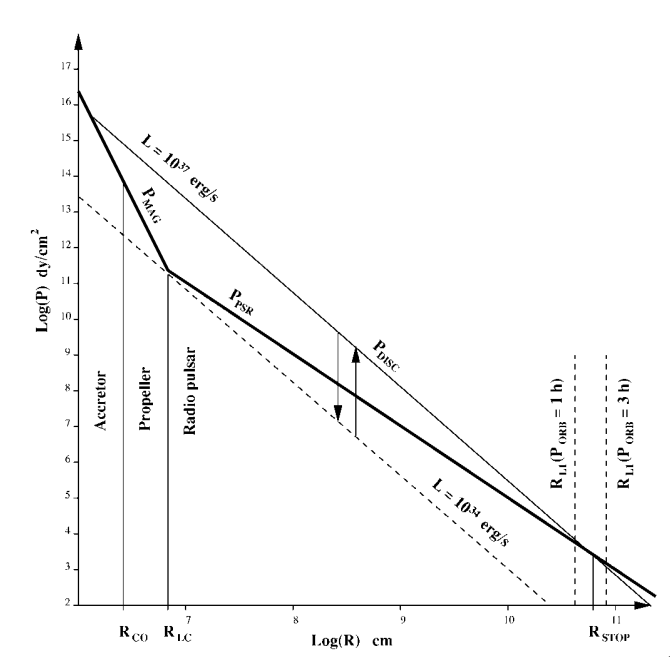
\includegraphics[width=0.6\linewidth]{Immagini/Grafico_pressione_raggio.png}
    \caption{Grafico pressione-raggio}
    \label{fig: grafico pressione raggio}
\end{figure}
Ora, la pressione di un disco di accrescimento si può calcolare come pressione di ariete $P_{ram} = \rho v_{ff}^2$ esercitata dalla materia in caduta libera.
In particolare, la pressione del disco sarà $\propto P_{ram}$.
Occorre quindi calcolare la velocità di caduta libera $v_{ff} = \frac{2GM}{R}$, e usare l'equazione di continuità $\rho v_{ff}^2 \cdot4\pi r^2 = \dot{M} \xrightarrow{} \rho = \frac{\dot{M}}{4\pi R^2} \left(\frac{R}{2GM}\right)^{1/2} $: infine, la pressione sarà
\begin{equation}
    \rho v_{ff}^2 = \frac{\dot{M}}{4\pi R^2}\left( \frac{R}{2GM} \right)^{\frac{1}{2}}\left( \frac{R}{2GM} \right)^{-1} \propto \dot{M}M^{1/2}R^{-5/2},
\end{equation}
che viene rappresentata nella \textbf{Figura \ref{fig: grafico pressione raggio}} come la riga tratteggiata con pendenza $-5/2 = -2,5$, che salirebbe o scenderebbe (nella figura è già all'altezza minima che può raggiungere) a seconda che $\dot{M}$ cresca o diminuisca.
Questo significa che, fissato il resto, a seconda del valore di $\dot{M}$, $R_m$ assumerà valori diversi, che si posizioneranno in punti diversi rispetto agli altri raggi (che sono invece fissati), il ché comporterà NS con comportamenti diversi!
Si noti che la retta tratteggiata più bassa è quella che passa per il punto di intersezione fra l'andamento dettato da $P_{mag}$ e quello dettato da $P_{rad}$: da questo punto in giù non ci sono più punti di equilibrio.
Se prima le intersezioni di $P_D$ (pressione del disco) con $P_{mag}$ e $P_{rad} $ erano punti stabili, questo ultimo punto è instabile.
La pressione magnetica crolla molto rapidamente, quindi se interseca la pressione del disco lì si ha un nuovo equilibrio: $P_{mag} = P_D$. 
Questo è esattamente (concettualmente) come il \textit{limite di Chandrasekhar}: la radiazione spazza via tutto quanto finché non si giunge a $P_{mag} = P_D$. 
Se però $P_D$ scende al limite, poiché la pressione di radiazione libera lo spazio attorno e la stella è libera di emettere radio, si può passare da \textit{accrescitore} a \textbf{radio ejector}, dove appunto la zona intorno al disco è completamente ripulita.
Nel grafico in \textbf{Figura \ref{fig: grafico pressione raggio}}, la situazione di Radio Ejector corrisponderebbe alla parte a destra di $R_{LC}$ nel caso della retta tratteggiata più bassa.
\footnote{Una pulsar il cui accrescimento è inibito da questa emissione è stata trovata, e se ne discute in \cite{Burderi_2002}}

\subsubsection{Archaeopteryx}
In sistemi binari, il campo magnetico dopo tempi secolari varia, e dopo che la pulsar a un certo punto si spegnerà, può avvenire una tracimazione dal lobo di Roche (Roche Overflow), e che la compagna quindi inizi a perdere materia che, spiraleggiando, formerà un disco di accrescimento.
Una volta che la compagna finisce la materia da dare, tornando a dimensioni normali, l'accrescimento si interrompe, spegnendo nuovamente la NS.
Questo overflow è intermittente, e non se ne conosce la ragione; ciò tuttavia permette di trovare sistemi che mostrino entrambi i comportamenti delle due fasi, facendo così da "anello di congiunzione".

\subsection{Sistemi binari}

\subsubsection{Forze mareali}
Le forze di marea in genere sono del tipo
\begin{equation}
    F_{mar} = \frac{GMml}{R^3},
    \label{eq: forze mareali}
\end{equation}
dove se $l$, la dimensione dell'oggetto su cui agisce la forza, decresce, o $R$, la distanza da esso, cresce, la forza sarà piccola.
Se due corpi orbitano a una distanza sufficientemente piccola, come nel caso di due stelle che interagiscono per accrescimento, le forze mareali sono influenti!
Gli oggetti tenderanno ad allungarsi lungo la congiungente.
D'altronde, i due corpi del sistema binario ruoteranno anche ognuno attorno al proprio asse.
Le NS hanno raggi minuscoli, e sono estremamente compatte, per cui non subiranno marea se non proprio negli ultimissimi momenti prima del merger.
La stella compagna, d'altra parte, se il sistema non è troppo largo, deformerà eccome, e nel mentre ruoterà attorno al proprio asse:
laddove si forma il "bulge" dovuto alle forze di marea, la materia che ruota attorno all'asse della compagna periodicamente si adatta alla forma di esso, per poi tornare a contrarsi una volta superato.
Questo movimento è frutto del lavoro svolto dalla forza di marea, che si disperde: la stella si scalda, ed emette radiazione, perdendo quindi energia ma non momento angolare.
Ricordiamo che in un sistema binario l'energia è proporzionale al semiasse maggiore dell'orbita, mentre il momento angolare alla sua area: se il momento angolare resta costante, allora l'area deve rimanere costante.
A parità di momento angolare, sistemi binari con energie diverse hanno semiassi maggiori diversi: $E_1>E_2 \xrightarrow{} a_1>a_2$.
Se, quindi, ho un sistema binario con un momento angolare fissato, questo perdendo energia tenderà all'ellissi con il semiasse maggiore più piccolo (minimizzando l'energia), cioè il \textit{cerchio}: questo fenomeno prende il nome di \textbf{circolarizzazione}.
Minimizzando ancora di più l'energia, la frequenza di rotazione della compagna attorno al proprio asse diventa uguale alla velocità angolare del sistema, e mostrerà così alla NS sempre la stessa faccia; questo fenomeno prende il nome di \textbf{sincronizzazione}.\footnote{Si noti che la luna, in effetti, è sincronizzata con la terra, ed è pure leggermente allungata lungo la direzione congiungente!}

\subsubsection{Potenziale di Roche}
Nel sistema di riferimento rotante del centro di massa (CM) di un sistema binario, le due stelle sembrano ferme. 
Tuttavia, questo s.d.r. sta in effetti ruotando, e quindi ci saranno fenomeni legati al fatto che non sia inerziale: forza \textbf{centrifuga} e forza di \textbf{Coriolis}.
Finché oltre la rotazione non ci sono moti, le forze di Coriolis sono nulle, e possiamo concentrarci sulla forza centrifuga: questa dipenderà solamente dalla posizione.
Se mi metto nel punto di vista in cui tutto sembra fermo, posso definire il \textbf{potenziale di Roche}.
Per farlo, dobbiamo considerare tutti e tre i potenziali: due gravitazionali e uno dovuto alla forza centrifuga
\begin{equation}
    U(r) = -\frac{GM_1}{r_1} - \frac{GM_2}{r_2} - \frac{\Omega^2r^2}{2},
\end{equation}
dove abbiamo che $r_1$ ed $r_2$ sono le distanze del punto in cui stiamo valutando il potenziale rispetto ai due oggetti del sistema, mentre $r$ è la distanza dal CM.
\begin{figure}[h!]
    \centering
    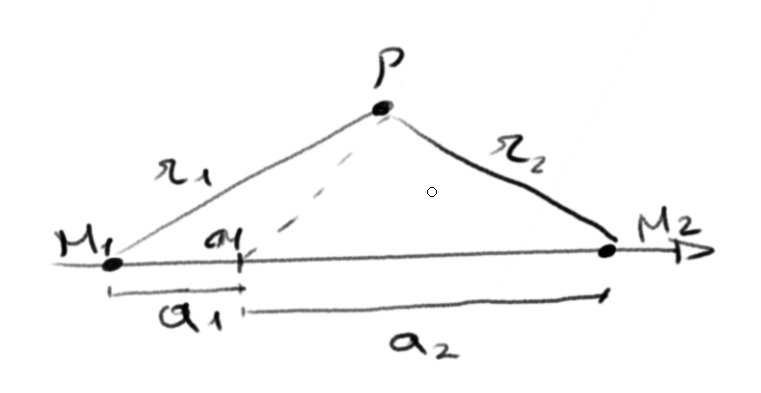
\includegraphics[width=0.5\linewidth]{Immagini/potensiale di roche su punto.png}
    % \caption{Caption}
    \label{fig: potenziale di Roche su un punto P}
\end{figure}\\
Definiamo altre due quantità: $a_1$ sarà la distanza del primo oggetto dal CM, mentre $a_2$ la distanza dal CM del secondo.

\subsubsection{Punti Lagrangiani}
A questo punto prendiamo il caso particolare in cui il punto si trovi lungo l'asse congiungente:
\begin{figure}[h!]
    \centering
    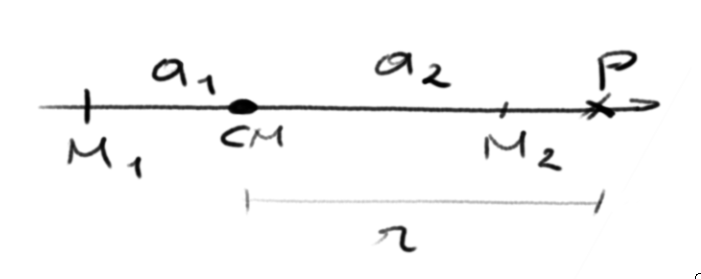
\includegraphics[width=0.5\linewidth]{Immagini/potenziale di Roche lungo asse congiungente.png}
    % \caption{Caption}
    \label{fig: Potenziale di Roche lungo congiungente}
\end{figure}\\
In questo caso noto che $r_1 = a_1 + r$, $r_2 = r - a_2$, per cui
\begin{equation}
    F(r, \theta=0)= -\frac{GM_1}{(a_1+r)^2} - \frac{GM_2}{(r-a_2)^2} + \Omega^2r \xrightarrow{impongo}=0,
\end{equation}
dove imponendo che la forza sia uguale a zero si troveranno i 5 zeri corrispondenti all'equazione di V grado che abbiamo scritto.
Ognuno di questi zeri sarà un punto \textbf{Lagrangiano}, di equilibrio:
$L_3$ dietro la stella più pesante, $L_2$ dietro la più leggera, $L_1$ tra le due, e infine $L_4$ ed $L_5$ che si trovano ai vertici di un triangolo equilatero la cui base è la separazione fra le due masse.
I punti Lagrangiani sono punti di equilibrio \textit{instabile}.
Nei punti $L_4$ ed $L_5$ tuttavia, se un oggetto si dovesse spostare leggermente acquistando una velocità rispetto al sistema in rotazione, le forze di Coriolis agiscono perpendicolarmente alla direzione del moto, generando così un moto oscillatorio attorno al punto Lagrangiano, chiamato \textbf{orbita a trottola}, o \textbf{tadpole orbit}.
Questo effetto rende l'equilibrio effettivamente stabile: la forza di Coriolis agisce un po' come una molla che riporta l'oggetto vicino alla sua posizione.
È come se il sistema “auto-correggesse” gli spostamenti, non perché c'è una forza diretta che tira verso il punto, ma perché il moto risultante è tale da farlo orbitare stabilmente lì attorno.
Si definisce per comodità una quantità che prende il nome di "\textbf{mass ratio}", caratteristica di ogni sistema binario:
\begin{equation}
    q = \frac{m_2}{m_1}<1,
\end{equation}
dove per convenzione $m_1$ è la massa dell'oggetto più massivo dei due.
Con il mass ratio, si può scrivere
\begin{equation}
    a_1 = a\frac{q}{1+q}\xrightarrow{q\xrightarrow{}0} qa.
\end{equation}
Si noti che per sistemi così sbilanciati, cioè per $q$ piccoli, un oggetto che si trovi in $L_4,L_5$ è come se ruotasse attorno a $M_1$.\footnote{Poiché nei punti $L_4$ ed $L_5$ del sistema terra luna non c'è niente, sono punti fantastici per mettere dei satelliti in orbita.}
Si definiscono come \textbf{Lobi di Roche} le superfici di \textit{isopotenziale} che passano per $L_1$, oltre il quale si ricade nella zona di influenza dell'altra stella.
A questo punto se la stella compagna evolve verso la fase di gigante rossa, come del latte messo a bollire che inizia a fare schiuma comincerà a strabordare, attraverso $L_1$, cedendo materiale alla zona di influenza della NS, causando il "\textbf{roche lobe overflow}".
A causa delle forze di Coriolis, la materia che cade verso la compagna avrà una velocità, e quindi spiraleggierà seguendo un'ellissi, che la porterà, dopo aver fatto almeno un giro completo, a scontrarsi nuovamente con la nuova materia in ingresso da $L_1$, e facendo ciò disperde ulteriormente energia (ma non momento angolare), circolarizzando sempre di più.
Dopo un po' si raggiunge un'orbita circolare a un certo raggio, e entrano in gioco le forze viscose: queste causano una perdita di momento angolare, per cui alcune orbite cadono più dentro e altre vanno verso fuori, formando così una struttura a disco.\footnote{Si noti che tutto ciò è dovuto al fatto che $L_1$ è un punto che sta ruotando!}

\subsubsection{Tidal torque interaction}
A tutto ciò si aggiunge poi il torque mareale che agisce sul bulge che ruota e cerca di allontanarsi dalla congiungente, che restituisce il momento angolare trasferito verso l'esterno del disco alla stella compagna: \textbf{tidal torque interaction}.
L'altra parte del momento angolare, invece, è quella che cade sulla primaria, e che ne causa lo \textit{spin up}.
Si definiscono i \textbf{raggi di Roche} come il raggio di una sfera di volume equivalente: 
% si noti infatti che andando verso i poli la forza centrifuga sarà minore, per una questione geometrica, e i lobi saranno deformati per questo motivo.
i lobi infatti sono chiaramente deformati, in particolare con una forma allungata lungo la congiungente; se $M_1>>M_2$ il lobo sarà poco deformato, ma se le masse sono confrontabili, entrambi i lobi saranno ben deformati.
Ora, a uno scambio di massa attraverso l'overflow si verificano delle variazioni nei parametri orbitali, quindi se capisco come variano le orbite, so 
a priori come variano i lobi di Roche, e posso dedurre se la tracimazione può avvenire o meno.
